% Options for packages loaded elsewhere
\PassOptionsToPackage{unicode}{hyperref}
\PassOptionsToPackage{hyphens}{url}
\PassOptionsToPackage{dvipsnames,svgnames*,x11names*}{xcolor}
%
\documentclass[
  graybox,natbib,nospthms]{svmono}
\usepackage{amsmath,amssymb}
\usepackage{lmodern}
\usepackage{ifxetex,ifluatex}
\ifnum 0\ifxetex 1\fi\ifluatex 1\fi=0 % if pdftex
  \usepackage[T1]{fontenc}
  \usepackage[utf8]{inputenc}
  \usepackage{textcomp} % provide euro and other symbols
\else % if luatex or xetex
  \usepackage{unicode-math}
  \defaultfontfeatures{Scale=MatchLowercase}
  \defaultfontfeatures[\rmfamily]{Ligatures=TeX,Scale=1}
  \setmonofont[Scale=0.7]{Source Code Pro}
\fi
% Use upquote if available, for straight quotes in verbatim environments
\IfFileExists{upquote.sty}{\usepackage{upquote}}{}
\IfFileExists{microtype.sty}{% use microtype if available
  \usepackage[]{microtype}
  \UseMicrotypeSet[protrusion]{basicmath} % disable protrusion for tt fonts
}{}
\makeatletter
\@ifundefined{KOMAClassName}{% if non-KOMA class
  \IfFileExists{parskip.sty}{%
    \usepackage{parskip}
  }{% else
    \setlength{\parindent}{0pt}
    \setlength{\parskip}{6pt plus 2pt minus 1pt}}
}{% if KOMA class
  \KOMAoptions{parskip=half}}
\makeatother
\usepackage{xcolor}
\IfFileExists{xurl.sty}{\usepackage{xurl}}{} % add URL line breaks if available
\IfFileExists{bookmark.sty}{\usepackage{bookmark}}{\usepackage{hyperref}}
\hypersetup{
  pdftitle={An Open Compendium of Soil Datasets},
  pdfauthor={Tomislav Hengl (OpenGeoHub)},
  colorlinks=true,
  linkcolor=Maroon,
  filecolor=Maroon,
  citecolor=Blue,
  urlcolor=Blue,
  pdfcreator={LaTeX via pandoc}}
\urlstyle{same} % disable monospaced font for URLs
\usepackage[paperwidth=18.90cm, paperheight=24.58cm, top=2.1cm, bottom=2.1cm, inner=2cm, outer=2cm]{geometry}
\usepackage{longtable,booktabs,array}
\usepackage{calc} % for calculating minipage widths
% Correct order of tables after \paragraph or \subparagraph
\usepackage{etoolbox}
\makeatletter
\patchcmd\longtable{\par}{\if@noskipsec\mbox{}\fi\par}{}{}
\makeatother
% Allow footnotes in longtable head/foot
\IfFileExists{footnotehyper.sty}{\usepackage{footnotehyper}}{\usepackage{footnote}}
\makesavenoteenv{longtable}
\usepackage{graphicx}
\makeatletter
\def\maxwidth{\ifdim\Gin@nat@width>\linewidth\linewidth\else\Gin@nat@width\fi}
\def\maxheight{\ifdim\Gin@nat@height>\textheight\textheight\else\Gin@nat@height\fi}
\makeatother
% Scale images if necessary, so that they will not overflow the page
% margins by default, and it is still possible to overwrite the defaults
% using explicit options in \includegraphics[width, height, ...]{}
\setkeys{Gin}{width=\maxwidth,height=\maxheight,keepaspectratio}
% Set default figure placement to htbp
\makeatletter
\def\fps@figure{htbp}
\makeatother
\setlength{\emergencystretch}{3em} % prevent overfull lines
\providecommand{\tightlist}{%
  \setlength{\itemsep}{0pt}\setlength{\parskip}{0pt}}
\setcounter{secnumdepth}{5}
\usepackage{amsmath} % if desired
\usepackage{unicode-math}
%\setmathfont{latinmodern-math.otf}
\usepackage{float}
\usepackage{color}
\usepackage{fancyvrb}
\usepackage{longtable}
\usepackage{booktabs}
\usepackage{graphicx}
\providecommand{\tightlist}{\setlength{\itemsep}{0pt}\setlength{\parskip}{0pt}}
\usepackage[hyphens]{url}
\usepackage{hyperref}
%\usepackage{fontspec}
%\setsansfont{Roboto}[
%  Path = fonts/Roboto/,
%  Extension = .ttf,
%  UprightFont = *-Regular,
%  %-- Upright --%
%  FontFace={ul}{n}{Font=*-Thin},
%  FontFace={l}{n}{Font=*-Light},
%  FontFace={m}{n}{Font=*-Regular},
%  FontFace={mb}{n}{Font=*-Medium},
%  FontFace={b}{n}{Font=*-Bold},
%  FontFace={eb}{n}{Font=*-Black},
%  % %-- Italic --%
%  FontFace={ul}{it}{Font=*-ThinItalic},
%  FontFace={l}{it}{Font=*-LightItalic},
%  FontFace={m}{it}{Font=*-Italic},
%  FontFace={mb}{it}{Font=*-MediumItalic},
%  FontFace={b}{it}{Font=*-BoldItalic},
%  FontFace={eb}{it}{Font=*-BlackItalic},
%]

% Place links in parens
\renewcommand{\href}[2]{#2 (\url{#1})}
% Use auto ref for internal links
\let\oldhyperlink=\hyperlink
\renewcommand{\hyperlink}[2]{\autoref{#1}}
\def\chapterautorefname{Chapter}
\def\sectionautorefname{Section}
\def\subsectionautorefname{Section}
\def\subsubsectionautorefname{Section}

\setlength{\emergencystretch}{3em}  % prevent overfull lines
\vbadness=10000 % suppress underfull \vbox
\hbadness=10000 % suppress underfull \vbox
\hfuzz=10pt

\usepackage{framed,color}
\definecolor{shadecolor}{RGB}{231,231,231}

\renewcommand{\textfraction}{0.05}
\renewcommand{\topfraction}{0.8}
\renewcommand{\bottomfraction}{0.8}
\renewcommand{\floatpagefraction}{0.75}

\renewenvironment{quote}{\begin{VF}}{\end{VF}}
\let\oldhref\href
\renewcommand{\href}[2]{#2\footnote{\url{#1}}}

\let\BeginKnitrBlock\begin \let\EndKnitrBlock\end

\ifxetex
  \usepackage{letltxmacro}
  \setlength{\XeTeXLinkMargin}{1pt}
  \LetLtxMacro\SavedIncludeGraphics\includegraphics
  \def\includegraphics#1#{% #1 catches optional stuff (star/opt. arg.)
    \IncludeGraphicsAux{#1}%
  }%
  \newcommand*{\IncludeGraphicsAux}[2]{%
    \XeTeXLinkBox{%
      \SavedIncludeGraphics#1{#2}%
    }%
  }%
\fi

\makeatletter
\newenvironment{kframe}{%
\medskip{}
\setlength{\fboxsep}{.8em}
 \def\at@end@of@kframe{}%
 \ifinner\ifhmode%
  \def\at@end@of@kframe{\end{minipage}}%
  \begin{minipage}{\columnwidth}%
 \fi\fi%
 \def\FrameCommand##1{\hskip\@totalleftmargin \hskip-\fboxsep
 \colorbox{shadecolor}{##1}\hskip-\fboxsep
     % There is no \\@totalrightmargin, so:
     \hskip-\linewidth \hskip-\@totalleftmargin \hskip\columnwidth}%
 \MakeFramed {\advance\hsize-\width
   \@totalleftmargin\z@ \linewidth\hsize
   \@setminipage}}%
 {\par\unskip\endMakeFramed%
 \at@end@of@kframe}
\makeatother

\makeatletter
\@ifundefined{Shaded}{
}{\renewenvironment{Shaded}{\begin{kframe}}{\end{kframe}}}
\makeatother

\newenvironment{rmdblock}[1]
  {
  % \begin{itemize}
  % \renewcommand{\labelitemi}{
  %   \raisebox{-.7\height}[0pt][0pt]{
  %     {\setkeys{Gin}{width=3em,keepaspectratio}\includegraphics{images/#1}}
  %   }
  % }
  % \setlength{\fboxsep}{10em}
  \begin{kframe}
  % \item
  }
  {
  \end{kframe}
  % \end{itemize}
  }
\newenvironment{rmdnote}
  {\begin{rmdblock}{note}}
  {\end{rmdblock}}
\newenvironment{rmdcaution}
  {\begin{rmdblock}{caution}}
  {\end{rmdblock}}
\newenvironment{rmdimportant}
  {\begin{rmdblock}{important}}
  {\end{rmdblock}}
\newenvironment{rmdtip}
  {\begin{rmdblock}{tip}}
  {\end{rmdblock}}
\newenvironment{rmdwarning}
  {\begin{rmdblock}{warning}}
  {\end{rmdblock}}

\usepackage{makeidx}
\makeindex
\ifluatex
  \usepackage{selnolig}  % disable illegal ligatures
\fi
\usepackage[]{natbib}
\bibliographystyle{spbasic}

\title{An Open Compendium of Soil Datasets}
\author{Tomislav Hengl (OpenGeoHub)}
\date{11 May, 2021}

\begin{document}
\maketitle

%\cleardoublepage\newpage\thispagestyle{empty}\null
%\cleardoublepage\newpage\thispagestyle{empty}\null
%\cleardoublepage\newpage
\thispagestyle{empty}
\begin{center}
% \includegraphics{images/dedication.pdf}
\end{center}

\setlength{\abovedisplayskip}{-5pt}
\setlength{\abovedisplayshortskip}{-5pt}

{
\hypersetup{linkcolor=}
\setcounter{tocdepth}{1}
\tableofcontents
}
\hypertarget{about}{%
\chapter{About}\label{about}}

\hypertarget{rationale}{%
\section{Rationale}\label{rationale}}

This is a public compendium of global, regional, national and
sub-national \textbf{soil samples} and/or \textbf{soil profile} datasets (points with
Observations and Measurements of soil properties and characteristics).
Datasets listed here, assuming compatible open license, are afterwards
imported into the \href{https://gitlab.com/openlandmap/}{\textbf{Global compilation of soil chemical and physical
properties and soil classes}} and
eventually used to create a better open soil information across countries.
The specific objectives of this initiative are:

\begin{itemize}
\tightlist
\item
  To enable data digitization, import and binding + harmonization,\\
\item
  To accelerate research collaboration and networking,\\
\item
  To enable development of more accurate / more usable global and
  regional soil property and class maps (typically published via
  \url{https://OpenLandMap.org}),
\end{itemize}

The minimum requirements to submit a dataset for inclusion to \href{https://gitlab.com/openlandmap/}{the
OpenLandMap repository} are:

\begin{itemize}
\tightlist
\item
  License and terms of use clearly specified AND,\\
\item
  Complete and consistent metadata that can ensure correct
  standardization and harmonization steps AND,\\
\item
  At least 50 unique spatial locations AND,\\
\item
  No broken or invalid URLs,
\end{itemize}

Datasets that do NOT satisfy the above listed minimum requirements might be
removed. If you discover an issue with license, data description or
version number of a dataset, please open a \href{https://github.com/OpenGeoHub/SoilSamples/issues}{Github
issue}.

Recommended settings for all datasets are:

\begin{itemize}
\tightlist
\item
  Peer-reviewed versions of the datasets (i.e.~a dataset accompanied
  with a peer-reviewed publication) should have the priority,\\
\item
  Register your dataset (use e.g.~\url{https://zenodo.org}) and assign a DOI
  to each version,\\
\item
  Provide enough metadata so that it can be imported and bind with
  other data without errors,\\
\item
  If your dataset is a compilation of previously published datasets, please
  indicate in the description,
\end{itemize}

Information outdated or missing? Please open an issue or best do a
correction and then a \href{https://docs.github.com/en/github/collaborating-with-issues-and-pull-requests/creating-a-pull-request}{pull
request}.

\begin{figure}
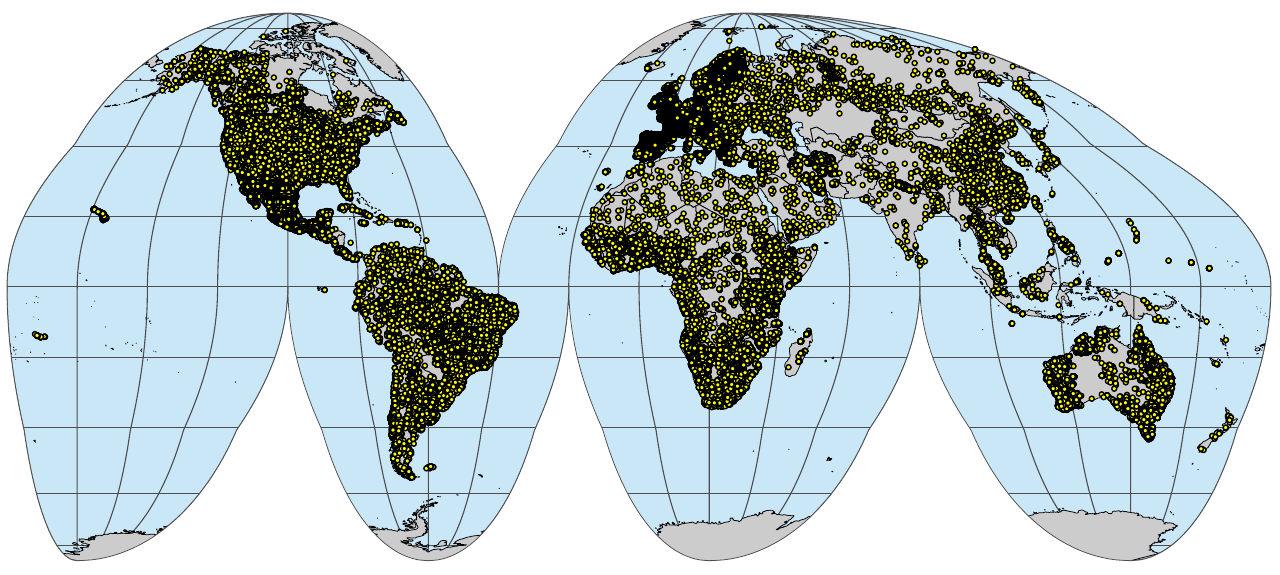
\includegraphics[width=1\linewidth]{img/sol_chem.pnts_sites} \caption{Soil profiles and soil samples with chemical and physical properties global compilation. For more info see: https://gitlab.com/openlandmap/compiled-ess-point-data-sets.}\label{fig:soil-pnts}
\end{figure}

Soil variables of interest include:

\begin{enumerate}
\def\labelenumi{\arabic{enumi}.}
\tightlist
\item
  \textbf{Chemical soil properties}:
\end{enumerate}

\begin{itemize}
\tightlist
\item
  Soil organic carbon, total carbon, total nitrogen,
\item
  Soil pH, effective Cation Exchange Capacity (eCEC),
\item
  Macro-nutrients: extractable --- potassium (K), calcium (Ca), sodium
  (Na), magnesium (Mg) and similar,
\item
  Micro-nutrients: phosphorus (P), sulfur (S), iron (Fe), zinc (Zn)
  and similar,
\item
  Soil pollutants, heavy metals and similar,
\item
  Electrical conductivity,
\end{itemize}

\begin{enumerate}
\def\labelenumi{\arabic{enumi}.}
\setcounter{enumi}{1}
\tightlist
\item
  \textbf{Physical soil properties}:
\end{enumerate}

\begin{itemize}
\tightlist
\item
  Texture fractions: silt, clay and sand, stone content,
\item
  Bulk density, depth to bedrock and similar,
\item
  Hydraulic conductivity, water content, water holding capacity and
  similar,
\item
  Soil temperature,
\end{itemize}

\begin{enumerate}
\def\labelenumi{\arabic{enumi}.}
\setcounter{enumi}{2}
\tightlist
\item
  \textbf{Soil biological / biodiversity variables}:
\end{enumerate}

\begin{itemize}
\tightlist
\item
  Soil biomass,
\item
  Soil micro-, meso-, macro- and mega-fauna abundance,
\item
  Soil biodiversity indices,
\end{itemize}

\begin{enumerate}
\def\labelenumi{\arabic{enumi}.}
\setcounter{enumi}{3}
\tightlist
\item
  \textbf{Soil classification / taxonomy variables}:
\end{enumerate}

\begin{itemize}
\tightlist
\item
  Soil type,
\item
  Soi suitability classes,
\item
  Soil texture classes and families,
\end{itemize}

\begin{enumerate}
\def\labelenumi{\arabic{enumi}.}
\setcounter{enumi}{4}
\tightlist
\item
  \textbf{Soil absorbances / soil spectroscopy variables}:
\end{enumerate}

\begin{itemize}
\tightlist
\item
  Soil absorbance in VIS-NIR and MIR part of spectra,
\end{itemize}

This document is based on the \url{https://www.bigbookofr.com/} repository
by Oscar Baruffa.

\hypertarget{recommended-columns}{%
\section{Recommended columns}\label{recommended-columns}}

As a general rule of thumb we recommend all contributors to use the following
general scheme to organize Soil Observations \& Measurements with three main tables
and metadata + legends organized in other tables:

\begin{figure}
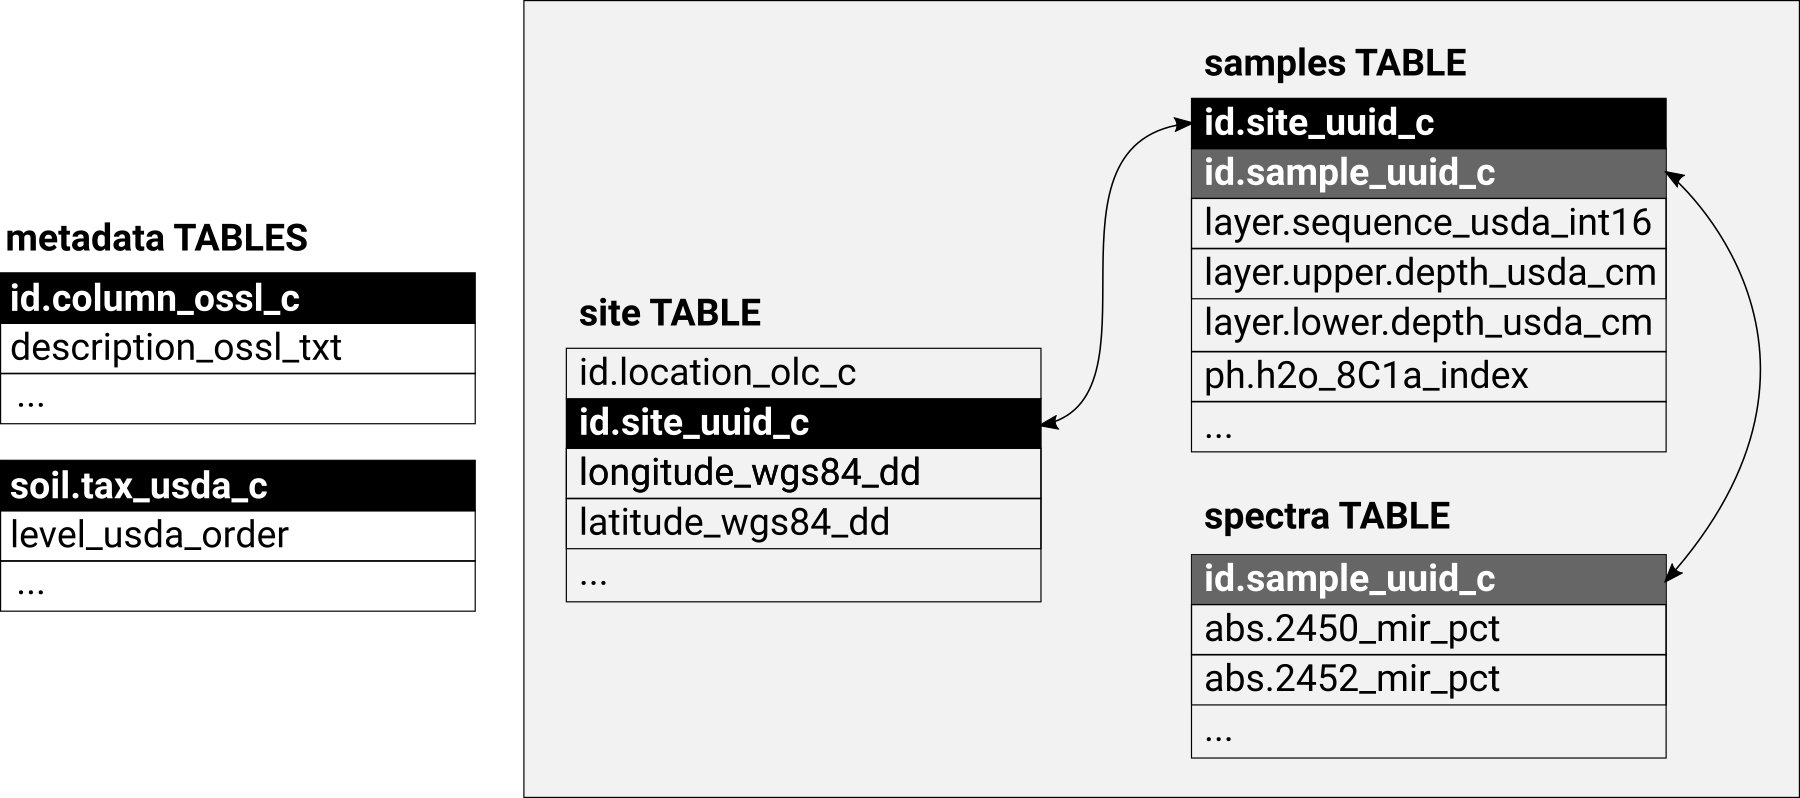
\includegraphics[width=1\linewidth]{img/design_soil_om_sheme} \caption{Recommended soil profiles and soil samples database schema.}\label{fig:soil-db}
\end{figure}

We recommend using the USDA \href{https://ncsslabdatamart.sc.egov.usda.gov/}{National Cooperative Soil Survey (NCSS) Soil
Characterization Database} codes and specification as much as possible. These are explained in detail in the \href{https://www.nrcs.usda.gov/Internet/FSE_DOCUMENTS/stelprdb1253872.pdf}{\textbf{Kellogg Soil Survey Laboratory Methods Manual}}.

For the \textbf{site} table please use (at least) the following columns:

\begin{enumerate}
\def\labelenumi{\arabic{enumi}.}
\tightlist
\item
  Unique site ID generated using some UUID generator tool; example: \texttt{id.site\_uuid\_c\ =\ \textquotesingle{}672d1fd6-b186-11eb-8a61-7446a0925130\textquotesingle{}}\\
\item
  Unique \href{https://opensource.google/projects/open-location-code}{Open Location Codes} ID which identifies the site location; example: \texttt{id.location\_olc\_c\ =\ \textquotesingle{}84MVX5FH+PJ\textquotesingle{}}\\
\item
  \href{https://www.ogc.org/standards/om}{Observation OGC} schema title; example: \texttt{observation.ogc.schema.title\_ogc\_txt\ =\ \textquotesingle{}Open\ Soil\ Spectroscopy\ Library\textquotesingle{}}\\
\item
  \href{https://www.ogc.org/standards/om}{Observation OGC} schema URL; example: \texttt{observation.ogc.schema\_idn\_url\ =\ \textquotesingle{}\textquotesingle{}}\\
\item
  Observation date begin; example: \texttt{observation.date.begin\_iso.8601\_yyyy.mm.dd\ =\ \textquotesingle{}2000.02.10\textquotesingle{}}\\
\item
  Observation date end; example: \texttt{observation.date.end\_\ iso.8601\_yyyy.mm.dd\ =\ \textquotesingle{}2000.02.10\textquotesingle{}}\\
\item
  Location address as Street and number, Local postcode, Town, County, State; example: \texttt{location.address\_utf8\_txt\ =\ \textquotesingle{}\textquotesingle{}}\\
\item
  Country(ies) the data was/were collected; example: \texttt{location.country\_iso.3166\_c\ =\ \textquotesingle{}USA\textquotesingle{}}\\
\item
  Location method e.g.~GPS; example: \texttt{location.method\_any\_c\ =\ \textquotesingle{}GPS\textquotesingle{}}\\
\item
  Field surveyor title or organization; example: \texttt{surveyor.title\_utf8\_txt\ =\ \textquotesingle{}USDA\ Natural\ Resource\ Conservation\ Service\ (NRCS)\ staff\textquotesingle{}}\\
\item
  Field surveyor contact email; example: \texttt{surveyor.contact\_ietf\_email\ =\ \textquotesingle{}support@usda.gov\textquotesingle{}}\\
\item
  Field surveyor address as Street and number, Local postcode, Town, County, State; example: \texttt{surveyor.address\_utf8\_txt\ =\ \textquotesingle{}USDA-NRCS-NSSC,\ Federal\ Building,\ Room\ 152,\ Mail\ Stop,\ 100\ Centennial\ Mall\ North,\ Lincoln,\ NE\textquotesingle{}}\\
\item
  Site \href{https://spatialreference.org/ref/epsg/wgs-84/}{WGS84 longitude} coordinate; example: \texttt{longitude\_wgs84\_dd\ =\ \textquotesingle{}-122.8208847\textquotesingle{}}\\
\item
  Site \href{https://spatialreference.org/ref/epsg/wgs-84/}{WGS84 latitude} coordinate; example: \texttt{latitude\_wgs84\_dd\ =\ \textquotesingle{}43.9742584\textquotesingle{}}\\
\item
  Approximate location error (for GPS coordinates use 30 m); example: \texttt{location.error\_any\_m\ =\ \textquotesingle{}30\textquotesingle{}}\\
\item
  Title of the dataset; example: \texttt{dataset.title\_utf8\_txt\ =\ \textquotesingle{}Kellog\textquotesingle{}s\ lab\ SSL\textquotesingle{}}\\
\item
  Code identification of the dataset; example: \texttt{dataset.code\_ascii\_txt\ =\ \textquotesingle{}KSSL\textquotesingle{}}\\
\item
  The URL address of the dataset web page; example: \texttt{dataset.address\_idn\_url\ =\ \textquotesingle{}https://ncsslabdatamart.sc.egov.usda.gov/\textquotesingle{}}\\
\item
  Data license title for the dataset; example: \texttt{dataset.license.title\_ascii\_txt\ =\ \textquotesingle{}CC-0\textquotesingle{}}\\
\item
  Data license URL for the dataset; example: \texttt{dataset.license.address\_idn\_url\ =\ \textquotesingle{}https://creativecommons.org/share-your-work/public-domain/cc0/\textquotesingle{}}\\
\item
  International DOI foundation code for the corresponding dataset version; example: \texttt{dataset.doi\_idf\_c\ =\ \textquotesingle{}10.2136/sssaj2019.06.0205\textquotesingle{}}\\
\item
  Person responsible for the dataset; example: \texttt{dataset.contact.name\_utf8\_txt\ =\ \textquotesingle{}Richard\ R.\ Ferguson\textquotesingle{}}
  Email contact of the person responsible for the dataset; example: \texttt{dataset.contact.email\_ietf\_email\ =\ \textquotesingle{}support@usda.gov\textquotesingle{}}\\
\item
  Local dataset ID of the site; example: \texttt{id.dataset.site\_ascii\_c\ =\ \textquotesingle{}603\textquotesingle{}}\\
\item
  Local user assigned ID of the site; example: \texttt{id.user.site\_ascii\_c\ =\ \textquotesingle{}01-DRJ-01\textquotesingle{}}\\
\item
  Unique project code; example: \texttt{id.project\_ascii\_c\ =\ \textquotesingle{}TEX18\textquotesingle{}}\\
\end{enumerate}

For the \textbf{samples} table please use some of the columns:

\begin{enumerate}
\def\labelenumi{\arabic{enumi}.}
\tightlist
\item
  Unique site ID generated using some UUID generator tool; example: \texttt{id.site\_uuid\_c\ =\ \textquotesingle{}672d1fd6-b186-11eb-8a61-7446a0925130\textquotesingle{}}\\
\item
  Unique sample ID generated using some UUID generator tool; example: \texttt{id.sample\_uuid\_c\ =\ \textquotesingle{}31d454be-b1ac-11eb-8a61-7446a0925130\textquotesingle{}}\\
\item
  Layer sequence number; example: \texttt{layer.sequence\_usda\_uint16\ =\ \textquotesingle{}11\textquotesingle{}}\\
\item
  Layer type; example: \texttt{layer.type\_usda\_c\ =\ \textquotesingle{}horizon\textquotesingle{}}\\
\item
  Layer field label used e.g.~for soil samples; example: \texttt{layer.field.label\_any\_c\ =\ \textquotesingle{}S00OR-039-001-2\textquotesingle{}}\\
\item
  Layer upper depth in cm; example: \texttt{layer.upper.depth\_usda\_cm\ =\ \textquotesingle{}13\textquotesingle{}}\\
\item
  Layer lower depth in cm; example: \texttt{layer.lower.depth\_usda\_cm\ =\ \textquotesingle{}36\textquotesingle{}}\\
\item
  Layer horizon designation based on USDA system; example: \texttt{horizon.designation\_usda\_c\ =\ \textquotesingle{}A2\textquotesingle{}}\\
\item
  Layer horizon designation disconituity based on USDA system; example: \texttt{horizon.designation.discontinuity\_usda\_c\ =\ \textquotesingle{}\textquotesingle{}}\\
\item
  Layer horizon structure type based on USDA system; example: \texttt{layer.structure.type\_usda\_c\ =\ \textquotesingle{}\textquotesingle{}}\\
\item
  Layers horizon structure grade based on the USDA system; example: \texttt{layer.structure.grade\_usda\_c\ =\ \textquotesingle{}\textquotesingle{}}\\
\item
  Layer texture class based on the USDA system; example: \texttt{layer.texture\_usda\_c\ =\ \textquotesingle{}Gravelly\ Clay\textquotesingle{}}\\
\item
  Sand content; description: \texttt{sand.tot\_3a1a1a\_wpct} = Total sand is the soil separate with 0.05 to 2.0 mm article diameter. It is reported a gravimetric percent on a \textless2 mm base. H prep.\\
\item
  Silt content; description: \texttt{silt.tot\_3a1a1a\_wpct} = Total silt is the soil separate with 0.002 to 0.05 mm particle size. It is reported as a gravimetric percent on a \textless2 mm base.\\
\item
  Clay content; description: \texttt{clay.tot\_3a1a1a\_wpct} = Total clay is the soil separate with \textless0.002 mm particle diameter. Clay size carbonate is included. Total clay is reported as a weight percent of the \textless2 mm fraction.\\
\item
  Coarse Fragments, Greater 2mm, ; description: \texttt{wpg2\_3a2\_wpct} = The gravimetric percentage of greater than 2 mm diameter particles reported on a whole soil base.\\
\item
  Water Retention, 15 Bar, \textless2mm, Air-dry; description: \texttt{wr.1500kbar\_3c2a1a.b\_wpct} = 15 bar water on air dry soil is the gravimetric water content of \textless2 mm air dry samples after equilibration at 15 bars water tension. It is reported on a \textless2 mm base. The value is influenced by clay \%, mineralogy, and organic carbon \%.\\
\item
  Water Retention, 1/3 Bar, \textless2mm Clod; description: \texttt{wr.33kbar\_3c1a.e1a\_wpct} = 1/3 bar water, clods is the gravimetric percent water in natural fabric (clods) after equilibration at 1/3 bar water tension. It is reported on a \textless2 mm base.\\
\item
  Aggregate stability; description: \texttt{aggstb\_1b1b2a1\_wpct} = Aggregate stability is the weight percent of 0.5mm - 2mm aggregates remaining after wet sieving.
\item
  Bulk density clod, \textless2 mm fraction, 1/3 bar; description: \texttt{bd.clod\_3b1a\_gcm3} = Bulk density, \textless2 mm fraction, 1/3 bar is the weight per unit volume of the \textless2 mm fraction, with volume being measured after equilibration at 1/3 bar water tension. It is reported as grams per cubic centimeter on a \textless2 mm base.\\
\item
  Bulk density, core, \textless2 mm fraction; description: \texttt{bd.core\_3b4a\_gcm3} = Bulk density, \textless2mm fraction, field moist is the weight per unit volume of the \textless2 mm fraction, with volume measured at field (sampling) moisture. Measurements are made on known volume cores. It is reported as grams per cubic centimeter, \textless2 mm base.\\
\item
  Total carbon; description: \texttt{c.tot\_4h2a1.3a1\_wpct} = Total carbon is a measure of all organic and inorganic carbon, including that found in carbonate minerals.\\
\item
  Total nitrogen; description: \texttt{n.tot\_4h2a1.3a1\_wpct} = Total nitrogen is a measure of all organic and inorganic nitrogen, including that found in nitrogen minerals.\\
\item
  Total sulfur; description: \texttt{s.tot\_4h2a1.3a1\_wpct} = Total sulfur is a measure of all organic and inorganic sulfur, including that found in sulfide minerals.\\
\item
  Total organic carbon; description: \texttt{oc.tot\_est.calc\_wpct} = Estimated Organic Carbon based on Total C, GP prep.\\
\item
  Total organic carbon based on dry combustion; description: \texttt{oc.tot\_4h2a1.3a1\_wpct} = CMS analyte. Organic carbon is a measure of all organic forms of carbon in the soil, including organic carbon within minerals.
\item
  Effervescence, 1N HCl; description: \texttt{na2co3.pres\_1b1b2d4\_class} = The visual effervescence of the prepared sample when treated with 1N HCl.\\
\item
  Calcium carbonate content; description: \texttt{caco3\_4e1a1a1a1.2\_wpct} = Carbonate in the \textless{} 2mm fraction is measured by CO2 evolution after acid treatment. It is reported as gravimetric percent CaCO3 on a \textless2 mm base, even though carbonates of Mg, Na, K, and Fe may be present and react with the acid.\\
\item
  Calcium, NH4OAc Extractable, 2M KCl displacement; description: \texttt{ca.ext\_4b1a1b1.4a.b1\_cmolkg} = NH4OAC extractable calcium is the fraction removed by pH 7.0 NH4OAC. It is assumed to represent the exchangeable Ca. It is reported as meq per 100 grams on a \textless2 mm base. It is not reported for samples containing carbonates or soluble salts.\\
\item
  CEC, NH4OAc, pH 7.0, 2M KCl displacement; description: \texttt{pcec.ext\_4b1a1a1a1a.b1\_cmolkg} = CEC by NH4OAC is the cation exchange capacity of the sample, determined by 1N NH4OAC in a system highly buffered at pH 7.0 The NH4 is displaced by 2M KCl to obtain a solution without solids. It is reported as meq per 100 grams sample, on a \textless2 mm base.\\
\item
  Magnesium, NH4OAc Extractable, 2M KCl displacement; description: \texttt{mg.ext\_4b1a1b1.4a.b1\_cmolkg} = NH4OAC extractable magnesium is the fraction removed by pH 7.0 NH4OAC. It is assumed to represent the exchangeable Mg if MgCO3 is not present. It is reported as meq per 100 grams on a \textless2 mm base.\\
\item
  Potassium, NH4OAc Extractable, 2M KCl displacement; description: \texttt{k.ext\_4b1a1b1.4a.b1\_cmolkg} = NH4OAC extractable potassium is the fraction removed by pH 7.0 NH4OAC. It is assumed to represent the exchangeable K. It is reported as meq per 100 grams on a \textless2 mm base.\\
\item
  Sodium, NH4OAc Extractable, 2M KCl displacement; description: \texttt{na.ext\_4b1a1b1.4a.b1\_cmolkg} = NH4OAC extractable sodium is the fraction removed by pH 7.0 NH4OAC. It is assumed to represent the exchangeable Na. It is reported as meq per 100 grams on a \textless2 mm base.\\
\item
  Iron, ammonium oxalate extractable; description: \texttt{fe.ox\_4g2a1a1.5a.b1\_wpct} = Ammonium oxalate extractable iron is considered a measure of the noncrystalline Fe in soils. It provides some inferences of the amount of Fe in various forms. It is reported as gravimetric \% on a \textless2mm base.\\
\item
  Iron, dithinoite-citrate extractable; description: \texttt{fe.dith\_4g1b1.4a.b1\_wpct} = Dithionite citrate extractable iron is considered a general measure of total pedogenic iron. It provides inferences on the amount of iron in various forms, P fixing potential, aggregate stability, and degree of weathering. Reported as grav \% on \textless2mm.\\
\item
  Iron, sodium pyrophosphate extractable; description: \texttt{fe.pyp\_4g3a1.3a.b1\_wpct} = Sodium pyrophosphate extractable iron is assumed to be the fraction associated with organic complexes. It is reported as gravimetric percent on a \textless2 mm base.\\
\item
  Aluminum, ammonium oxalate extractable; description: \texttt{al.ox\_4g2a1a1.5a.b1\_wpct} = Ammonium oxalate extractable aluminum is an estimate of the total pedogenic Al, much of which may be in noncrystalline materials or complexed by organic matter. It is reported as gravimetric percent on a \textless2 mm base.\\
\item
  Aluminum, dithinoite-citrate extractable; description: \texttt{al.dith\_4g1b1.4a.b1\_wpct} = Dithionite citrate extractable aluminum is an indicator of the amount of aluminum substituted for iron in iron oxides. It does not necessarily represent total pedogenic Al.\\
\item
  Aluminum, sodium pyrophosphate extractable; description: \texttt{al.pyp\_4g3a1.3a.b1\_wpct} = Sodium pyrophosphate extractable aluminum is the fraction extracted by 0.1M sodium pyrophosphate. It was originally considered the portion associated with organic compounds, although subsequent evidence indicates other forms are also removed.\\
\item
  Aluminum, KCl extractable; description: \texttt{al.kcl\_4b3b1a1.b1\_cmolkg} = KCl extractable aluminum approximates the exchangeable Al, and is a measure of the active acidity present in soils with a 1:1 water pH less than 5.5. It relates to the immediate lime requirement and the CEC of the soil.\\
\item
  Aluminum, ammonium oxalate extractable; description: \texttt{al.ox\_4g2a1a1.5a.b1\_wpct} = Ammonium oxalate extractable aluminum is an estimate of the total pedogenic Al, much of which may be in noncrystalline materials or complexed by organic matter. It is reported as gravimetric percent on a \textless2 mm base.\\
\item
  Aluminum, dithinoite-citrate extractable; description: \texttt{al.dith\_4g1b1.4a.b1\_wpct} = Dithionite citrate extractable aluminum is an indicator of the amount of aluminum substituted for iron in iron oxides. It does not necessarily represent total pedogenic Al.\\
\item
  Aluminum, sodium pyrophosphate extractable; description: \texttt{al.pyp\_4g3a1.3a.b1\_wpct} = Sodium pyrophosphate extractable aluminum is the fraction extracted by 0.1M sodium pyrophosphate. It was originally considered the portion associated with organic compounds, although subsequent evidence indicates other forms are also removed.\\
\item
  Aluminum, KCl extractable; description: \texttt{al.kcl\_4b3b1a1.b1\_cmolkg} = KCl extractable aluminum approximates the exchangeable Al, and is a measure of the active acidity present in soils with a 1:1 water pH less than 5.5. It relates to the immediate lime requirement and the CEC of the soil.\\
\item
  Base saturation, NH4OAc, pH7; description: \texttt{bsat\_4b4c1\_pct} = NH4OAC base saturation (pH 7.0) is calculated by (BASE\_SUM/CEC\_NH4)*100.\\
\item
  Aluminum saturation; description: \texttt{alsat\_4b4d1a\_pct} = Aluminum saturation is calculated by (AL\_KCL/(Sum of bases))*100. It provides some inference of potential Al toxicity problems, although many other factors influence Al toxicity.\\
\item
  Soil pH 1:1 water; description: \texttt{ph.h2o\_4c1a2a1a.b1\_index} = The pH, 1:1 soil-water suspension is the pH of a sample measured in distilled water at a 1:1 soil:solution ratio. If wider ratios increase the pH, salts are indicated.\\
\item
  Soil pH 1:2 0.01-M calcium choride; description: \texttt{ph.cacl2\_4c1a2a2a.b1\_index} = The pH, 1:2 soil-CaCl2 is the pH of a sample measured in 0.01M CaCl2 at a 1:2 soil:solution ratio.\\
\item
  Electrical Conductivity, Predict, 1:2 (w/w); description: \texttt{ec.w\_4f1b1a1\_dsm} = The salt predict electrical conductivity is used to determine whether additional salt analyses are needed, and to estimate appropriate dilution ratios for additional tests. It is reported as mmhos per centimeter of a 1:2 soil:water mixture by weight.\\
\item
  Electrical Conductivity, Saturation Extract; description: \texttt{ec.ext.sat\_4f2b1a1\_dsm} = Electrical Conductivity, Saturation Extract
\item
  Sodium adsorption ratio; description: \texttt{sodium.ads.ratio\_4f3b\_index} = The sodium absorption ratio is calculated by NA\_SATX/sqrt((CA\_SATX+MG\_SATX)/2). It is approximately equal to the exchangeable sodium percentage.\\
\item
  Exchangeable sodium percentage saturated; description: \texttt{na.exch\_4f3a2\_pct} = This is the exchangeable sodium percentage (ESP), reported on a \textless2 mm base. If salts are present, ESP has been corrected for the water soluble Na.\\
\item
  Corrected Gypsum, \textless{} 2mm; description: \texttt{gyp\_4e2b1a1a1.2\_wpct} = Corrected Gypsum ( Uncorrected Gypsum * Factor)\\
\item
  Phosphorus, Mehlich3 extractable; description: \texttt{p.meh3\_4d6a1a.b1\_mgkg} = The phosphorus extracted by the Mehlich III solution.\\
\item
  Phosphorus, Olsen extractable; description: \texttt{p.olsn\_4d5a1a.b1\_mgkg} = The Olsen extractable phosphorus is used as an indicator of available phosphorus in calcareous soil materials (pH \textgreater6).
\end{enumerate}

For the \textbf{spectra} table please use the following columns:

\begin{enumerate}
\def\labelenumi{\arabic{enumi}.}
\tightlist
\item
  Unique sample ID generated using some UUID generator tool; example: \texttt{id.sample\_uuid\_c\ =\ \textquotesingle{}31d454be-b1ac-11eb-8a61-7446a0925130\textquotesingle{}}\\
\item
  Layer field label used e.g.~for soil samples; example: \texttt{layer.field.label\_any\_c\ =\ \textquotesingle{}S00OR-039-001-2\textquotesingle{}}\\
\item
  Aborbance per wavelength e.g.~\texttt{a.w2450\_mir\_pct}\\
  \ldots{}\\
\end{enumerate}

\hypertarget{contributing}{%
\section{Contributing}\label{contributing}}

Please feel free to contribute entries. See \href{https://github.com/OpenGeoHub/SoilSamples}{GitHub
repository} for more detailed
instructions.

\hypertarget{contributors}{%
\section{Contributors}\label{contributors}}

If you've contribute, add also your name and Twitter, ORCID or blog link
below:

\href{https://twitter.com/tom_hengl}{Tomislav Hengl}, \href{https://twitter.com/sandersoil}{Jonathan Sanderman}, \href{https://orcid.org/0000-0002-9788-9947}{Mario Antonio Guevara
Santamaria},

\hypertarget{disclaimer}{%
\section{Disclaimer}\label{disclaimer}}

The data is provided ``as is''. \href{https://opengeohub.org/about}{OpenGeoHub foundation} and its suppliers and licensors hereby disclaim all warranties of any kind, express or implied, including, without limitation, the warranties of merchantability, fitness for a particular purpose and non-infringement. Neither OpenGeoHub foundation nor its suppliers and licensors, makes any warranty that the Website will be error free or that access thereto will be continuous or uninterrupted. You understand that you download from, or otherwise obtain content or services through, the Website at your own discretion and risk.

\hypertarget{licence}{%
\section{Licence}\label{licence}}

This website/book is free to use, and is licensed under the \href{https://creativecommons.org/licenses/by/3.0/}{Creative
Commons Attribution 3.0
License}.

\hypertarget{soil-spectroscopy-for-global-good}{%
\section{Soil Spectroscopy for Global Good}\label{soil-spectroscopy-for-global-good}}

\href{https://soilspectroscopy.org/}{\textbf{SoilSpec4GG}} is a USDA-funded \href{https://nifa.usda.gov/press-release/nifa-invests-over-7-million-big-data-artificial-intelligence-and-other}{Food and Agriculture Cyberinformatics
Tools Coordinated Innovation Network NIFA Award \#2020-67021-32467} project. It brings together soil
scientists, spectroscopists, informaticians, data scientists and
software engineers to overcome some of the current bottlenecks
preventing wider and more efficient use of soil spectroscopy. A series
of working groups will be formed to address topics including calibration
transfer, model choice, outreach \& demonstration, and use of
spectroscopy to inform global carbon cycle modeling. For more info refer
to: \url{https://soilspectroscopy.org/}

\hypertarget{about-opengeohub}{%
\section{About OpenGeoHub}\label{about-opengeohub}}

\textbf{OpenGeoHub foundation} is a non-for-profit research foundation
located in Wageningen, the Netherlands. We specifically promote
publishing and sharing of Open Geographical and Geoscientific Data,
using and developing Open Source Software and encouraging and empowering
under-represented researchers e.g.~those from ODA recipient countries
and female researchers. We believe that the key measure of quality of
research in all sciences (and especially in geographical information
sciences) is in transparency and reproducibility of the computer code
used to generate results (read more in: \href{https://opengeohub.medium.com/}{``Everyone has a right to know
what is happening with the planet''}).

Some other connected publications and initiatives describing collation
and import of legacy soil observations and measurements that might interest
you:

\begin{itemize}
\tightlist
\item
  Arrouays, D., Leenaars, J. G., Richer-de-Forges, A. C., Adhikari,
  K., Ballabio, C., Greve, M., \ldots{} \& Heuvelink, G. (2017). \href{https://doi.org/10.1016/j.grj.2017.06.001}{\textbf{Soil
  legacy data rescue via GlobalSoilMap and other international and
  national initiatives}}.
  GeoResJ, 14, 1-19.\\
\item
  Batjes, N. H., Ribeiro, E., van Oostrum, A., Leenaars, J., Hengl,
  T., \& de Jesus, J. M. (2017). \href{http://www.earth-syst-sci-data.net/9/1/2017/}{\textbf{WoSIS: providing standardised soil
  profile data for the world}}. Earth System Science Data, 9(1), 1. \url{https://doi.org/10.5194/essd-9-1-2017}~
\item
  Gupta, S., Hengl, T., Lehmann, P., Bonetti, S., \& Or, D. (2021). \href{https://doi.org/10.5194/essd-13-1593-2021}{\textbf{SoilKsatDB:
  global database of soil saturated hydraulic conductivity measurements for
  geoscience applications}}. Earth System Science Data, 13(4), 1593-1612.
  \url{https://doi.org/10.5194/essd-13-1593-2021}\\
\item
  Hengl, T., MacMillan, R.A., (2019). \href{https://soilmapper.org/}{\textbf{Predictive Soil Mapping with
  R}}. OpenGeoHub foundation, Wageningen, the
  Netherlands, 370 pages, \url{https://soilmapper.org}, ISBN:
  978-0-359-30635-0.\\
\item
  Ramcharan, A., Hengl, T., Beaudette, D., \& Wills, S. (2017). \href{https://doi.org/10.2136/sssaj2016.12.0421}{\textbf{A soil
  bulk density pedotransfer function based on machine learning: A case
  study with the NCSS soil characterization
  database}}. Soil Science
  Society of America Journal, 81(6), 1279-1287.
  \url{https://doi.org/10.2136/sssaj2016.12.0421}
\item
  Rossiter, D.G.,: \href{https://www.isric.org/explore/soil-geographic-databases}{\textbf{Compendium of Soil Geographical
  Databases}}.
\end{itemize}

\hypertarget{new-to-markdown.-start-here}{%
\chapter{New to markdown. Start here}\label{new-to-markdown.-start-here}}

\hypertarget{clone-add-reference-submit-merge-request}{%
\section{Clone, add reference, submit merge request\ldots{}}\label{clone-add-reference-submit-merge-request}}

To add a new dataset, please follow these steps:

\begin{enumerate}
\def\labelenumi{\arabic{enumi}.}
\tightlist
\item
  Click on the edit button on the book homepage,\\
\item
  Login to Github.com and select ``Start a pull-request'',\\
\item
  Add new references to \texttt{020-dataset\_list.Rmd} and save,\\
\item
  Commit and push and make a \href{https://docs.github.com/en/github/collaborating-with-issues-and-pull-requests/creating-a-pull-request}{pull
  request}.\\
\item
  Once received we will check it and if you have followed the instructions closely,
  the reference will appear in the document as soon as the code is merged with the master,\\
\end{enumerate}

\begin{figure}
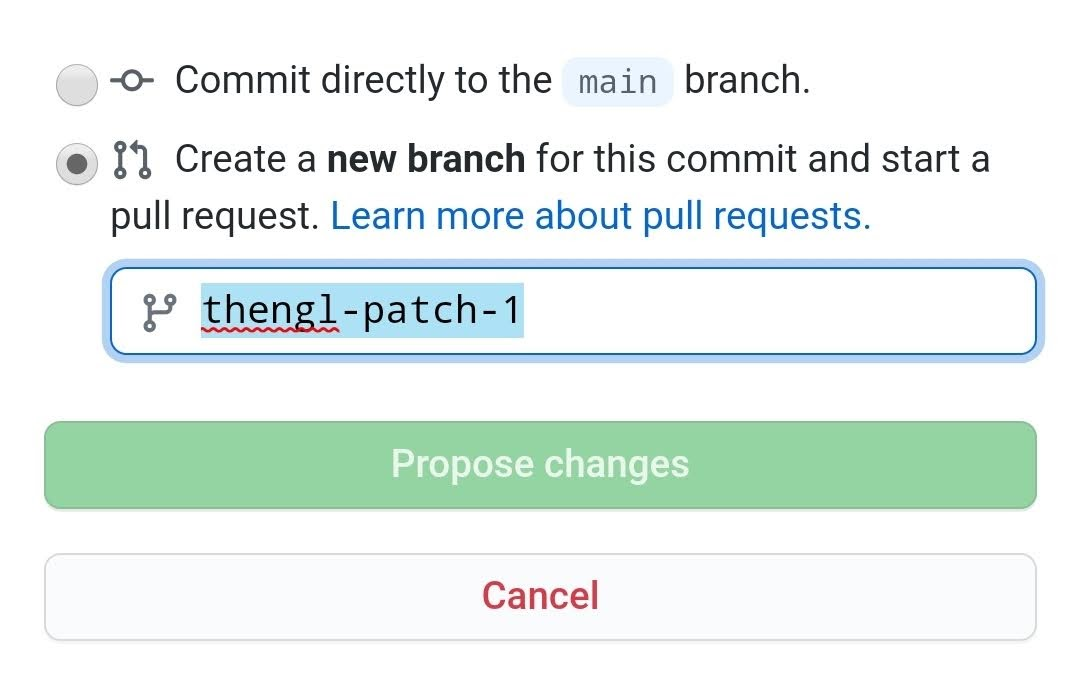
\includegraphics[width=0.5\linewidth]{img/example_pull_request} \caption{Example of a pull request on Github.com.}\label{fig:pull-request}
\end{figure}

If you're new to markdown and want to learn how to use it, please refer to \href{https://guides.github.com/features/mastering-markdown/}{this tutorial}.

If you are new to R and/or \href{https://pedometrics.org}{\textbf{pedometrics}}, please consider reading / installing:

\begin{itemize}
\tightlist
\item
  Kabacoff, R.I., (2011) \href{http://www.manning.com/kabacoff/}{``R in Action: Data Analysis and Graphics with R''}. Manning publications, ISBN: 9781935182399, 472 pages.
\item
  California Soil Resource Lab, (2017) \href{https://casoilresource.lawr.ucdavis.edu/software/}{``Open Source Software Tools for Soil Scientists''}, UC Davis.,\\
\item
  \href{http://www.rstudio.com/products/RStudio/}{RStudio},
\end{itemize}

If you'd like more of a roadmap to guide you through R, have a look at Oscar's blogpost:

\begin{itemize}
\tightlist
\item
  \url{https://oscarbaruffa.com/a-roadmap-for-getting-started-with-r/}
\end{itemize}

\hypertarget{video-course-getting-started-with-r}{%
\section{Video Course: Getting started with R}\label{video-course-getting-started-with-r}}

If you prefer video instruction with progress tracking:

\begin{itemize}
\tightlist
\item
  \url{https://rfortherestofus.com/courses/getting-started/}
\end{itemize}

\hypertarget{soil-data-communities-and-mailing-lists}{%
\chapter{Soil data communities and mailing lists}\label{soil-data-communities-and-mailing-lists}}

To follow progress of the soil data compilations consider connecting to some of the
active communities / registering for the mailing lists and/or discussion groups.

\hypertarget{pedometrics-community}{%
\section{Pedometrics community}\label{pedometrics-community}}

Pedometrics is the commission of the International Union of Soil Sciences. You can
read more about pedometrics from \textless www.pedometrics.org\textgreater. There is also \href{https://mailman.sydney.edu.au/mailman/listinfo/pedometrics}{Pedometrics
mailing list} where you
can ask more technical questions.

\hypertarget{digital-soil-mapping-community}{%
\section{Digital Soil Mapping community}\label{digital-soil-mapping-community}}

Digital Soil Mapping community (A Working Group of the International Union of Soil Sciences (IUSS))
can be accessed via the home page \textless www.digitalsoilmapping.org\textgreater{} and/or
via the Facebook group on \href{https://www.facebook.com/groups/DigitalSoilMapping}{Digital Soil Mapping}.

\hypertarget{datasets}{%
\chapter{Datasets}\label{datasets}}

\hypertarget{global-datasets}{%
\section{Global Datasets}\label{global-datasets}}

\hypertarget{fine-root-ecology-database-fred-compilation}{%
\subsection{Fine Root Ecology Database: FRED (compilation)}\label{fine-root-ecology-database-fred-compilation}}

\emph{Description}: Originally a plant root database but also contains some soil laboratory data
and soil observations.

\begin{itemize}
\tightlist
\item
  📕 Iversen CM, McCormack ML, Baer JK, Powell AS, Chen W, Collins C, Fan Y, Fanin N, Freschet GT, Guo D, Hogan JA, Kou L, Laughlin DC, Lavely E, Liese R, Lin D, Meier IC, Montagnoli A, Roumet C, See CR, Soper F, Terzaghi M, Valverde-Barrantes OJ, Wang C, Wright SJ, Wurzburger N, Zadworny M. (2021). \href{https://roots.ornl.gov/}{Fine-Root Ecology Database (FRED): A Global Collection of Root Trait Data with Coincident Site, Vegetation, Edaphic, and Climatic Data, Version 3}. Oak Ridge National Laboratory, TES SFA, U.S. Department of Energy, Oak Ridge, Tennessee, U.S.A.\\
\item
  🔗 Project website: \url{https://roots.ornl.gov/}\\
\item
  📂 Data download URL: \url{https://doi.org/10.25581/ornlsfa.014/1459186}\\
\item
  📍 Unique locations: 280\\
\item
  📋 Unique complete rows: 858\\
\item
  📝 Import steps: \href{https://gitlab.com/openlandmap/compiled-ess-point-data-sets/-/tree/master/themes/sol/SoilChemDB\#fine-root-ecology-database-fred}{chemsprops.FRED}
\end{itemize}

\hypertarget{global-harmonized-dataset-of-soc-change-under-perennial-crops-compilation}{%
\subsection{Global Harmonized Dataset of SOC change under perennial crops (compilation)}\label{global-harmonized-dataset-of-soc-change-under-perennial-crops-compilation}}

\emph{Description}: Soil Organic Carbon data from various publications. Many missing
years for PREVIOUS SOC and SOIL CHARACTERISTICS.

\begin{itemize}
\tightlist
\item
  📕 Ledo, A., Hillier, J., Smith, P. et al.~(2019) A global, empirical, harmonised dataset of soil organic carbon changes under perennial crops. Sci Data 6, 57. \url{https://doi.org/10.1038/s41597-019-0062-1}\\
\item
  🔗 Project website: \url{https://africap.info/}\\
\item
  📂 Data download URL: \url{https://doi.org/10.6084/m9.figshare.7637210.v2}\\
\item
  📍 Unique locations: 174\\
\item
  📋 Unique complete rows: 1526\\
\item
  📝 Import steps: \href{https://gitlab.com/openlandmap/compiled-ess-point-data-sets/-/tree/master/themes/sol/SoilChemDB\#global-harmonized-dataset-of-soc-change-under-perennial-crops}{chemsprops.SOCPDB}
\end{itemize}

\hypertarget{global-soil-respiration-db-compilation}{%
\subsection{Global Soil Respiration DB (compilation)}\label{global-soil-respiration-db-compilation}}

\emph{Description}: The database encompasses all published studies that report at least one of the following data measured in the field (not laboratory): annual soil respiration, mean seasonal soil respiration, a seasonal or annual partitioning of soil respiration into its source fluxes, soil respiration temperature response (Q10), or soil respiration at 10 degrees C.

\begin{itemize}
\tightlist
\item
  📕 Bond-Lamberty, B. and Thomson, A. (2010). A global database of soil respiration data, Biogeosciences, 7, 1915-1926, \url{https://doi.org/10.5194/bg-7-1915-2010}\\
\item
  🔗 Project website: \url{https://github.com/bpbond/srdb/}\\
\item
  📂 Data download URL: \url{https://github.com/bpbond/srdb/}\\
\item
  📍 Unique locations: 826\\
\item
  📋 Unique complete rows: 1596\\
\item
  📝 Import steps: \href{https://gitlab.com/openlandmap/compiled-ess-point-data-sets/-/tree/master/themes/sol/SoilChemDB\#global-soil-respiration-db}{chemsprops.SRDB}
\end{itemize}

\hypertarget{hydros-soil-hydraulic-functions-of-international-soils-compilation}{%
\subsection{HYDROS Soil hydraulic functions of international soils (compilation)}\label{hydros-soil-hydraulic-functions-of-international-soils-compilation}}

\emph{Description}: Contains a data base of 173 soil hydrological data (raw data) from 71 sites all over the world (Asia, Africa, Australia America and Europe). The samples were mainly collected and measured as part of research projects. The soils cover a wide range of texture classes and dry bulk densities. The data base consists of water retention and unsaturated hydraulic conductivity data.

\begin{itemize}
\tightlist
\item
  📕 Schindler, Uwe; Müller, Lothar (2015): \href{http://dx.doi.org/10.4228/ZALF.2003.273}{Soil hydraulic functions of
  international soils measured with the Extended Evaporation Method (EEM) and the HYPROP device}, Leibniz-Zentrum für Agrarlandschaftsforschung (ZALF) e.V.{[}\url{doi:10.4228/ZALF.2003.273}{]}\\
\item
  🔗 Project website:\\
\item
  📂 Data download URL: \url{http://dx.doi.org/10.4228/ZALF.2003.273}\\
\item
  📍 Unique locations: 71\\
\item
  📋 Unique complete rows: 173\\
\item
  📝 Import steps: \href{https://gitlab.com/openlandmap/compiled-ess-point-data-sets/-/tree/master/themes/sol/SoilHydroDB\#hydros}{chemsprops.HYDROS}
\end{itemize}

\hypertarget{isric-wise-harmonized-soil-profile-data-compilation}{%
\subsection{ISRIC WISE harmonized soil profile data (compilation)}\label{isric-wise-harmonized-soil-profile-data-compilation}}

\emph{Description}: ISRIC-WISE database holds selected site and horizon data for 10,250 soil profiles from 149 countries. Profile data were extracted from a wide range of sources and harmonized with respect to the original (1974) and revised (1988) Legend of the FAO-Unesco Soil Map of the World. Profiles have been described, sampled, and analyzed according to methods and standards in use in the originating countries. WISE was specifically developed for land-related applications at continental and global scales.

\begin{itemize}
\tightlist
\item
  📕 Batjes, N.H. (2019). \href{http://dx.doi.org/10.1111/j.1475-2743.2009.00202.x}{Harmonized soil profile data for applications at global and continental scales: updates to the WISE database}. Soil Use and Management 5:124-127. \url{DOI:10.1111/j.1475-2743.2009.00202.x}\\
\item
  🔗 Project website: \url{https:/isric.org}\\
\item
  📂 Data download URL: \url{https://files.isric.org/public/wise/WD-WISE.zip}\\
\item
  📍 Unique locations: 6723\\
\item
  📋 Unique complete rows: 23278\\
\item
  📝 Import steps: \href{https://gitlab.com/openlandmap/compiled-ess-point-data-sets/-/tree/master/themes/sol/SoilChemDB\#isric-wise-harmonized-soil-profile-data}{chemsprops.WISE}
\end{itemize}

\hypertarget{isric-world-soil-reference-collection}{%
\subsection{ISRIC World Soil Reference Collection}\label{isric-world-soil-reference-collection}}

\emph{Description}: World Soil Reference Collection comprises about 800 soil profiles
from over 70 countries with detailed soil profile and environmental data.

\begin{itemize}
\tightlist
\item
  📕 Batjes, N. H. (1995). \href{https://www.isric.org/sites/default/files/isric_report_1995_10b.pdf}{A homogenized soil data file for global
  environmental research: A subset of FAO, ISRIC and NRCS profiles (Version 1.0) (No.~95/10b)}. ISRIC. / Van de Ven, T., \& Tempel, P. (1994). \href{https://www.isric.org/sites/default/files/ISRIC_TechPap15b.pdf}{ISIS 4.0: ISRIC Soil Information System: User Manual}. ISRIC.\\
\item
  🔗 Project website: \url{https:/isis.isric.org}\\
\item
  📂 Data download URL: \url{https:/isis.isric.org}\\
\item
  📍 Unique locations: 785\\
\item
  📋 Unique complete rows: 5637\\
\item
  📝 Import steps: \href{https://gitlab.com/openlandmap/compiled-ess-point-data-sets/-/tree/master/themes/sol/SoilHydroDB\#isric-isis}{hydrosprops.ISIS}
\end{itemize}

\hypertarget{global-icrafisric-soil-spectroscopy-library-icrafisric}{%
\subsection{Global ICRAF/ISRIC Soil Spectroscopy Library --- (ICRAF/ISRIC)}\label{global-icrafisric-soil-spectroscopy-library-icrafisric}}

\emph{Description}: A Globally Distributed Soil Spectral Library Mid Infrared Diffuse
Reflectance Spectra. MIR scans for some 785 profiles from the ISRIC World Soil Reference Collection.
The samples are from 58 countries spanning Africa, Asia, Europe, North America, and South America.
Data available under the CC-BY 4.0 license.

\begin{itemize}
\tightlist
\item
  📕 World Agroforestry Centre, (2014). \href{https://worldagroforestry.org/sites/default/files/Description_ICRAF-ISRIC\%20Soil\%20VNIR\%20Spectral\%20Library.pdf}{The ICRAF/ISRIC spectral library}, Soil-Plant Spectral Diagnostics laboratory, United
  Nations Avenue, Nairobi, Kenya.\\
\item
  🔗 Project website: \url{https://www.worldagroforestry.org/sd/landhealth/soil-plant-spectral-diagnostics-laboratory/soil-spectra-library}\\
\item
  📂 Data download URL: \url{https://files.isric.org/public/other/ICRAF-ISRICVNIRSoilDatabase.zip}\\
\item
  📍 Unique locations: 785\\
\item
  📋 Unique complete rows:\\
\item
  📝 Import steps: \href{https://gitlab.com/soilspec4gg}{sslsprops.ICRAF\_ISRIC}
\end{itemize}

\hypertarget{global-database-of-soil-saturated-hydraulic-conductivity-measurements-ksat-compilation}{%
\subsection{Global database of soil saturated hydraulic conductivity measurements --- KSat (compilation)}\label{global-database-of-soil-saturated-hydraulic-conductivity-measurements-ksat-compilation}}

\emph{Description}: Contains a total of 13,258 Ksat measurements from 1908 sites were assembled from the published literature.

\begin{itemize}
\tightlist
\item
  📕 Gupta, S., Hengl, T., Lehmann, P., Bonetti, S., and Or, D.: (2021) \href{https://doi.org/10.5194/essd-13-1593-2021}{SoilKsatDB: global database of soil saturated hydraulic conductivity measurements for geoscience applications}, Earth Syst. Sci. Data, 13, 1593--1612, \url{https://doi.org/10.5194/essd-13-1593-2021}.\\
\item
  🔗 Project website:\\
\item
  📂 Data download URL: \url{https://doi.org/10.5281/zenodo.3752721}\\
\item
  📍 Unique locations: 1908\\
\item
  📋 Unique complete rows:\\
\item
  📝 Import steps: \href{https://gitlab.com/openlandmap/compiled-ess-point-data-sets/-/tree/master/themes/sol/SoilHydroDB}{hydrosprops}
\end{itemize}

\hypertarget{landpks-observations}{%
\subsection{LandPKS observations}\label{landpks-observations}}

\emph{Description}: Data collected by various people through the LandPKS App for mobile
phones (crowdsourced). Data is of limited quality and usually no laboratory data is collected and shared.

\begin{itemize}
\tightlist
\item
  📕 Herrick, J. E., Urama, K. C., Karl, J. W., Boos, J., Johnson, M. V. V., Shepherd, K. D., \ldots{} \& Kosnik, C. (2013). \href{https://doi.org/10.2489/jswc.68.1.5A}{The Global Land-Potential Knowledge System (LandPKS): Supporting Evidence-based, Site-specific Land Use and Management through Cloud Computing, Mobile Applications, and Crowdsourcing}. Journal of Soil and Water Conservation, 68(1), 5A-12A.\\
\item
  🔗 Project website: \url{http://portal.landpotential.org}\\
\item
  📂 Data download URL: \url{http://portal.landpotential.org/\#/landpksmap}\\
\item
  📍 Unique locations: 15326\\
\item
  📋 Unique complete rows: 41644\\
\item
  📝 Import steps: \href{https://gitlab.com/openlandmap/compiled-ess-point-data-sets/-/tree/master/themes/sol/SoilChemDB\#landpks-observations}{chemsprops.LandPKS}
\end{itemize}

\hypertarget{mangrove-forest-soil-db-compilation}{%
\subsection{Mangrove forest soil DB (compilation)}\label{mangrove-forest-soil-db-compilation}}

\emph{Description}: Point data set used to produce a global map of mangrove forest
soil carbon at 30 m spatial resolution.

\begin{itemize}
\tightlist
\item
  📕 Sanderman, J., Hengl, T., Fiske, G., Solvik, K., Adame, M. F., Benson, L., \ldots{} \& Duncan, C. (2018). \href{https://doi.org/10.1088/1748-9326/aabe1c}{A global map of mangrove forest soil carbon at 30 m spatial resolution}. Environmental Research Letters, 13(5), 055002.\\
\item
  🔗 Project website: \url{https://www.woodwellclimate.org/research-area/carbon/}\\
\item
  📂 Data download URL: \url{https://dataverse.harvard.edu/dataset.xhtml?persistentId=doi:10.7910/DVN/OCYUIT}\\
\item
  📍 Unique locations: 1568\\
\item
  📋 Unique complete rows: 7718\\
\item
  📝 Import steps: \href{https://gitlab.com/openlandmap/compiled-ess-point-data-sets/-/tree/master/themes/sol/SoilChemDB\#mangrove-forest-soil-db}{chemsprops.Mangroves}
\end{itemize}

\hypertarget{remnant-native-soc-database-compilation}{%
\subsection{Remnant native SOC database (compilation)}\label{remnant-native-soc-database-compilation}}

\emph{Description}: Soil carbon profile data from paired land use comparisons.

\begin{itemize}
\tightlist
\item
  📕 Sanderman, J., Hengl, T., \& Fiske, G. J. (2017). \href{https://doi.org/10.1073/pnas.1706103114}{Soil carbon debt of 12,000 years of human land use}. Proceedings of the National Academy of Sciences, 114(36), 9575-9580.\\
\item
  🔗 Project website: \url{https://www.woodwellclimate.org/research-area/carbon/}\\
\item
  📂 Data download URL: \url{https://doi.org/10.7910/DVN/QQQM8V/8MSBNI}\\
\item
  📍 Unique locations: 1604\\
\item
  📋 Unique complete rows: 224\\
\item
  📝 Import steps: \href{https://gitlab.com/openlandmap/compiled-ess-point-data-sets/-/tree/master/themes/sol/SoilChemDB\#remnant-native-soc-database}{chemsprops.RemnantSOC}
\end{itemize}

\hypertarget{soils-data-harmonization-database-sodah-compilation}{%
\subsection{SOils DAta Harmonization database: SoDaH (compilation)}\label{soils-data-harmonization-database-sodah-compilation}}

\emph{Description}: SoDaH is built on several network science efforts in the
United States. It's aim is to provide an open-access resource to facilitate and automate further harmonization and synthesis of soil carbon data.

\begin{itemize}
\tightlist
\item
  📕 Wieder, W. R., Pierson, D., Earl, S., Lajtha, K., Baer, S., Ballantyne, F., \ldots{} \& Weintraub, S. (2020). \href{https://doi.org/10.5194/essd-2020-195}{SoDaH: the SOils DAta Harmonization database, an open-source synthesis of soil data from research networks, version 1.0}. Earth System Science Data Discussions, 1-19. \url{https://doi.org/10.5194/essd-2020-195}\\
\item
  🔗 Project website: \url{https://lter.github.io/som-website}\\
\item
  📂 Data download URL: \url{https://doi.org/10.6073/pasta/9733f6b6d2ffd12bf126dc36a763e0b4}\\
\item
  📍 Unique locations: 1052\\
\item
  📋 Unique complete rows: 20383\\
\item
  📝 Import steps: \href{https://gitlab.com/openlandmap/compiled-ess-point-data-sets/-/tree/master/themes/sol/SoilChemDB\#soils-data-harmonization-database-sodah}{chemsprops.SoDaH}
\end{itemize}

\hypertarget{soil-health-db-compilation}{%
\subsection{Soil Health DB (compilation)}\label{soil-health-db-compilation}}

\emph{Description}: A database for global soil health assessment. Only limited soil properties
available.

\begin{itemize}
\tightlist
\item
  📕 Jian, J., Du, X., \& Stewart, R. D. (2020). A database for global soil health assessment. Scientific Data, 7(1), 1-8. \url{https://doi.org/10.1038/s41597-020-0356-3}.\\
\item
  🔗 Project website: \url{https://github.com/jinshijian/SoilHealthDB}\\
\item
  📂 Data download URL: \url{https://github.com/jinshijian/SoilHealthDB}\\
\item
  📍 Unique locations: 88\\
\item
  📋 Unique complete rows: 120\\
\item
  📝 Import steps: \href{https://gitlab.com/openlandmap/compiled-ess-point-data-sets/-/tree/master/themes/sol/SoilChemDB\#soil-health-db}{chemsprops.SoilHealthDB}
\end{itemize}

\hypertarget{soil-water-infiltration-global-database-swig-compilation}{%
\subsection{Soil Water Infiltration Global database --- SWIG (compilation)}\label{soil-water-infiltration-global-database-swig-compilation}}

\emph{Description}: Soil textural information (clay, silt, and sand content) is available for 3842 out of 5023 infiltration measurements.

\begin{itemize}
\tightlist
\item
  📕 Rahmati, M., Weihermüller, L., Vanderborght, J., Pachepsky, Y. A.,
  Mao, L., Sadeghi, S. H., \ldots{} \& Toth, B. (2018). \href{https://doi.org/10.5194/essd-10-1237-2018}{Development and analysis of the Soil Water Infiltration Global database}. Earth Syst. Sci. Data, 10, 1237--1263.\\
\item
  🔗 Project website:\\
\item
  📂 Data download URL: \url{https://doi.org/10.1594/PANGAEA.885492}\\
\item
  📍 Unique locations: 88\\
\item
  📋 Unique complete rows: 120\\
\item
  📝 Import steps: \href{https://gitlab.com/openlandmap/compiled-ess-point-data-sets/-/tree/master/themes/sol/SoilHydroDB\#swig}{chemsprops.SWIG}
\end{itemize}

\hypertarget{unsoda-unsaturated-soil-hydraulic-database-compilation}{%
\subsection{UNSODA Unsaturated Soil Hydraulic Database (compilation)}\label{unsoda-unsaturated-soil-hydraulic-database-compilation}}

\emph{Description}: The dataset contains measured soil water retention, hydraulic conductivity, and water diffusivity data, as well as pedological information of some 790 soil samples from around the world.

\begin{itemize}
\tightlist
\item
  📕 Nemes, Attila; Schaap, Marcel; Leij, Feike J.; Wösten, J. Henk M.
  (2015). \href{https://data.nal.usda.gov/dataset/unsoda-20-unsaturated-soil-hydraulic-database-database-and-program-indirect-methods-estimating-unsaturated-hydraulic-properties}{UNSODA 2.0: Unsaturated Soil Hydraulic Database. Database and program for indirect methods of estimating unsaturated hydraulic properties}. US Salinity Laboratory - ARS - USDA. \url{https://doi.org/10.15482/USDA.ADC/1173246}. / Børgesen, C. D., Jacobsen, O. H., Hansen, S., \& Schaap, M. G. (2006). Soil hydraulic properties near saturation, an improved conductivity model. Journal of Hydrology, 324(1-4), 40-50. \url{https://doi.org/10.1016/j.jhydrol.2005.09.014}
\item
  🔗 Project website:\\
\item
  📂 Data download URL: \href{https://data.nal.usda.gov/dataset/unsoda-20-unsaturated-soil-hydraulic-database-database-and-program-indirect-methods-estimating-unsaturated-hydraulic-properties}{Zip packages}\\
\item
  📍 Unique locations: 790\\
\item
  📋 Unique complete rows:\\
\item
  📝 Import steps: \href{https://gitlab.com/openlandmap/compiled-ess-point-data-sets/-/tree/master/themes/sol/SoilHydroDB\#unsoda}{hydrosprops.UNSODA}
\end{itemize}

\hypertarget{worldwide-organic-soil-carbon-and-nitrogen-data}{%
\subsection{Worldwide organic soil carbon and nitrogen data}\label{worldwide-organic-soil-carbon-and-nitrogen-data}}

\emph{Description}: A global point data set with organic soil carbon and nitrogen data.
Poor spatial location accuracy with error often \textgreater{} 10 km. Bulk density for many points has been
estimated not measured. Sampling year has not been but literature indicates:
1965, 1974, 1976, 1978, 1979, 1984. Most of samples come from natural vegetation (undisturbed) areas.

\begin{itemize}
\tightlist
\item
  📕 Zinke, P. J., Millemann, R. E., \& Boden, T. A. (1986). \href{https://cdiac.ess-dive.lbl.gov/ftp/ndp018/ndp018.pdf}{Worldwide organic soil carbon and nitrogen data}. Carbon Dioxide Information Center, Environmental Sciences Division, Oak Ridge National Laboratory.\\
\item
  🔗 Project website: \url{https://cdiac.ess-dive.lbl.gov/}\\
\item
  📂 Data download URL: \url{https://dx.doi.org/10.3334/CDIAC/lue.ndp018}\\
\item
  📍 Unique locations: 1712\\
\item
  📋 Unique complete rows: 3977\\
\item
  📝 Import steps: \href{https://gitlab.com/openlandmap/compiled-ess-point-data-sets/-/tree/master/themes/sol/SoilChemDB\#worldwide-organic-soil-carbon-and-nitrogen-data}{chemsprops.ISCND}
\end{itemize}

\hypertarget{africa}{%
\section{Africa}\label{africa}}

\hypertarget{africa-soil-profiles-database-compilation}{%
\subsection{Africa soil profiles database (compilation)}\label{africa-soil-profiles-database-compilation}}

\emph{Description}: A compilation of legacy soil profiles from hundreds of profiles.
Produced for the purpose of the Africa Soil Information Services (AfSIS) project.

\begin{itemize}
\tightlist
\item
  📕 Leenaars, J. G., Van Oostrum, A. J. M., \& Ruiperez Gonzalez, M. (2014). \href{https://www.isric.org/projects/africa-soil-profiles-database-afsp}{Africa soil profiles database version 1.2. A compilation of georeferenced and standardized legacy soil profile data for Sub-Saharan Africa (with dataset)}. Wageningen: ISRIC Report 2014/01; 2014.\\
\item
  🔗 Project website: \url{https://www.isric.org/projects/africa-soil-profiles-database-afsp}\\
\item
  📂 Data download URL: \url{https://data.isric.org/}\\
\item
  📍 Unique locations: 15630\\
\item
  📋 Unique complete rows: 60306\\
\item
  📝 Import steps: \href{https://gitlab.com/openlandmap/compiled-ess-point-data-sets/-/tree/master/themes/sol/SoilChemDB\#africa-soil-profiles-database}{chemsprops.AfSPDB}
\end{itemize}

\hypertarget{africa-soil-information-service-afsis1-soil-chemistry}{%
\subsection{Africa Soil Information Service (AfSIS1) Soil Chemistry}\label{africa-soil-information-service-afsis1-soil-chemistry}}

\emph{Description}: Soil spectroscopy-based soil samples datasets. Produced by World
Agroforestry Centre (ICRAF), Quantitative Engineering Design (QED), Center for
International Earth Science Information Network (CIESIN), The International Center
for Tropical Agriculture (CIAT), Crop Nutrition Laboratory Services (CROPNUTS) and
Rothamsted Research (RRES) for the purpose of the Africa Soil Information Services (AfSIS) project.
Many more samples have been collected in the period 2010--2018.

\begin{itemize}
\tightlist
\item
  📕 Towett, E. K., Shepherd, K. D., Tondoh, J. E., Winowiecki, L. A., Lulseged, T., Nyambura, M., \ldots{} \& Cadisch, G. (2015). Total elemental composition of soils in Sub-Saharan Africa and relationship with soil forming factors. Geoderma Regional, 5, 157-168. \url{https://doi.org/10.1016/j.geodrs.2015.06.002}\\
\item
  🔗 Project website: \url{https://github.com/qedsoftware/afsis-soil-chem-tutorial}\\
\item
  📂 Data download URL: \url{https://registry.opendata.aws/afsis/}\\
\item
  📍 Unique locations: 929\\
\item
  📋 Unique complete rows: 4162\\
\item
  📝 Import steps: \href{https://gitlab.com/openlandmap/compiled-ess-point-data-sets/-/tree/master/themes/sol/SoilChemDB\#africa-soil-information-service-afsis-soil-chemistry}{chemsprops.AfSIS1}
\end{itemize}

\hypertarget{asia}{%
\section{Asia}\label{asia}}

\hypertarget{northern-circumpolar-permafrost-soil-profiles-compilation}{%
\subsection{Northern circumpolar permafrost soil profiles (compilation)}\label{northern-circumpolar-permafrost-soil-profiles-compilation}}

\emph{Description}: Represents parts of Russian Federation and Canada.
This data set consists of significantly higher soil organic carbon concentrations.

\begin{itemize}
\tightlist
\item
  📕 Hugelius, G., Bockheim, J. G., Camill, P., Elberling, B., Grosse, G., Harden, J. W., \ldots{} \& Michaelson, G. (2013). \href{https://doi.org/10.5194/essd-5-393-2013}{A new data set for estimating organic carbon storage to 3 m depth in soils of the northern circumpolar permafrost region}. Earth System Science Data (Online), 5(2).\\
\item
  🔗 Project website: \url{https://bolin.su.se/data/ncscd/}\\
\item
  📂 Data download URL: \url{http://dx.doi.org/10.5879/ECDS/00000002}\\
\item
  📍 Unique locations: 410\\
\item
  📋 Unique complete rows: 7104\\
\item
  📝 Import steps: \href{https://gitlab.com/openlandmap/compiled-ess-point-data-sets/-/tree/master/themes/sol/SoilChemDB\#northern-circumpolar-permafrost-soil-profiles}{chemsprops.NCSCD}
\end{itemize}

\hypertarget{australia-oceania}{%
\section{Australia \& Oceania}\label{australia-oceania}}

\hypertarget{europe}{%
\section{Europe}\label{europe}}

\hypertarget{land-use-and-coverage-area-frame-survey-lucas-soil}{%
\subsection{Land Use and Coverage Area frame Survey: LUCAS soil}\label{land-use-and-coverage-area-frame-survey-lucas-soil}}

\emph{Description}: Top-soil samples only (0--20 cm). Currently there are three
campaigns with LUCAS soil samples: 2009, 2015 and 2018. This is currently the largest
systematic soil sample dataset for EU.

\begin{itemize}
\tightlist
\item
  📕 Orgiazzi, A., Ballabio, C., Panagos, P., Jones, A., \& Fernandez-Ugalde, O. (2018). \href{https://doi.org/10.1111/ejss.12499}{LUCAS Soil, the largest expandable soil dataset for Europe: a review}. European Journal of Soil Science, 69(1), 140-153.\\
\item
  🔗 Project website: \url{https://esdac.jrc.ec.europa.eu/content/lucas-2009-topsoil-data}\\
\item
  📂 Data download URL: \url{https://esdac.jrc.ec.europa.eu/content/lucas-2009-topsoil-data}\\
\item
  📍 Unique locations: 21272\\
\item
  📋 Unique complete rows: 21272 + 21859\\
\item
  📝 Import steps: \href{https://gitlab.com/openlandmap/compiled-ess-point-data-sets/-/tree/master/themes/sol/SoilChemDB\#lucas-soil}{chemsprops.LUCAS}
\end{itemize}

\hypertarget{gemas-2009}{%
\subsection{GEMAS 2009}\label{gemas-2009}}

\emph{Description}: Geochemical background and threshold for 53 chemical elements in
European agricultural soil.

\begin{itemize}
\tightlist
\item
  📕 Reimann, C., Fabian, K., Birke, M., Filzmoser, P., Demetriades, A., Negrel, P., \ldots{} \& Anderson, M. (2018). \href{https://doi.org/10.1016/j.apgeochem.2017.01.021}{GEMAS: Establishing geochemical background and threshold for 53 chemical elements in European agricultural soil}. Applied Geochemistry, 88, 302-318.\\
\item
  🔗 Project website: \url{http://gemas.geolba.ac.at/}\\
\item
  📂 Data download URL: \url{http://gemas.geolba.ac.at/}\\
\item
  📍 Unique locations: 4026\\
\item
  📋 Unique complete rows: 4131\\
\item
  📝 Import steps: \href{https://gitlab.com/openlandmap/compiled-ess-point-data-sets/-/tree/master/themes/sol/SoilChemDB\#gemas}{chemsprops.GEMAS}
\end{itemize}

\hypertarget{north-and-central-america}{%
\section{North and Central America}\label{north-and-central-america}}

\hypertarget{south-america}{%
\section{South America}\label{south-america}}

\hypertarget{sistema-de-informacion-de-suelos-de-latinoamerica-sislac-compilation}{%
\subsection{Sistema de Informacion de Suelos de Latinoamerica: SISLAC (compilation)}\label{sistema-de-informacion-de-suelos-de-latinoamerica-sislac-compilation}}

\emph{Description}: A compilation of legacy soil profiles from majority of Latin American
countries.

\begin{itemize}
\tightlist
\item
  📕 Alianza Mundial por el Suelo. 2013. Sistema de Informacion de Suelos de Latinoamerica (SISLAC). \url{https://hdl.handle.net/10568/49611}\\
\item
  🔗 Project website: \url{http://www.sislac.org/}\\
\item
  📂 Data download URL: \url{http://54.229.242.119/sislac/es}\\
\item
  📍 Unique locations: 14606\\
\item
  📋 Unique complete rows: 49994\\
\item
  📝 Import steps: \href{https://gitlab.com/openlandmap/compiled-ess-point-data-sets/-/tree/master/themes/sol/SoilChemDB\#sislac}{chemsprops.SISLAC}
\end{itemize}

\hypertarget{cifor-peatland-points-compilation}{%
\subsection{CIFOR peatland points (compilation)}\label{cifor-peatland-points-compilation}}

\emph{Description}: Peatland soil measurements (points) from the literature.

\begin{itemize}
\tightlist
\item
  📕 Murdiyarso, D., Roman-Cuesta, R. M., Verchot, L. V., Herold, M., Gumbricht, T., Herold, N., \& Martius, C. (2017). New map reveals more peat in the tropics (Vol. 189). CIFOR. \url{https://doi.org/10.17528/cifor/006452}\\
\item
  🔗 Project website: \url{https://www.cifor.org/}\\
\item
  📂 Data download URL:\\
\item
  📍 Unique locations:\\
\item
  📋 Unique complete rows: 756\\
\item
  📝 Import steps: \href{https://gitlab.com/openlandmap/compiled-ess-point-data-sets/-/tree/master/themes/sol/SoilChemDB\#cifor-peatland-points}{chemsprops.Peatlands}
\end{itemize}

\hypertarget{national-datasets}{%
\section{National Datasets}\label{national-datasets}}

\hypertarget{australia}{%
\subsection{Australia}\label{australia}}

\hypertarget{csiro-national-soil-site-database-compilation}{%
\subsubsection{CSIRO National Soil Site Database (compilation)}\label{csiro-national-soil-site-database-compilation}}

\emph{Description}: National legacy soil profile dataset. Compiled from various projects.

\begin{itemize}
\tightlist
\item
  📕 CSIRO (2020). CSIRO National Soil Site Database. v4. CSIRO. Data Collection. \url{https://data.csiro.au/collections/collection/CIcsiro:7526v004}.\\
\item
  🔗 Project website: \url{https://www.csiro.au/en/Do-business/Services/Enviro/Soil-archive}\\
\item
  📂 Data download URL: \url{https://doi.org/10.25919/5eeb2a56eac12}\\
\item
  📍 Unique locations: 13826\\
\item
  📋 Unique complete rows: 70791\\
\item
  📝 Import steps: \href{https://gitlab.com/openlandmap/compiled-ess-point-data-sets/-/tree/master/themes/sol/SoilChemDB\#csiro-national-soil-site-database}{chemsprops.NatSoil}
\end{itemize}

\hypertarget{belgium}{%
\subsection{Belgium}\label{belgium}}

\hypertarget{aardewerk-vlaanderen-2010}{%
\subsubsection{AARDEWERK-Vlaanderen-2010}\label{aardewerk-vlaanderen-2010}}

\emph{Description}: Legacy soil profile dataset for Flemish Region.

\begin{itemize}
\tightlist
\item
  📕 Beckers, V., Jacxsens, P., Van De Vreken, Ph., Van Meirvenne, M., Van Orshoven, J. (2011). Gebruik en installatie van de bodemdatabank AARDEWERK-Vlaanderen-2010. Spatial Applications Division Leuven, Belgium. / Ottoy, S., Beckers, V., Jacxsens, P., Hermy, M., \& Van Orshoven, J. (2015). \href{https://doi.org/10.1016/j.geoderma.2015.04.001}{Multi-level statistical soil profiles for assessing regional soil organic carbon stocks}. Geoderma, 253, 12-20. \url{https://doi.org/10.1016/j.geoderma.2015.04.001}\\
\item
  🔗 Project website: \url{https://www.dov.vlaanderen.be}\\
\item
  📂 Data download URL: \url{https://www.dov.vlaanderen.be}\\
\item
  📍 Unique locations: 6877
\item
  📋 Unique complete rows: 41310
\item
  📝 Import steps: \href{https://gitlab.com/openlandmap/compiled-ess-point-data-sets/-/tree/master/themes/sol/SoilChemDB\#aardewerk-vlaanderen-2010}{chemsprops.Vlaanderen2010}
\end{itemize}

\hypertarget{brazil}{%
\subsection{Brazil}\label{brazil}}

\hypertarget{a-national-soil-profile-database-for-brazil-compilation}{%
\subsubsection{A National Soil Profile Database for Brazil (compilation)}\label{a-national-soil-profile-database-for-brazil-compilation}}

\emph{Description}: National compilation of representative soil profiles. This dataset has been
used in FEBR. Data comes primarily from the Radam project (Projeto Radambrasil, 1973--1986).

\begin{itemize}
\tightlist
\item
  📕 Cooper, M., Mendes, L. M. S., Silva, W. L. C., \& Sparovek, G. (2005). \href{https://doi.org/10.2136/sssaj2004.0140}{A national soil profile database for Brazil available to international scientists}. Soil Science Society of America Journal, 69(3), 649-652. \url{https://doi.org/10.2136/sssaj2004.0140} / Benedetti, M. M., Curi, N., Sparovek, G., Carvalho Filho, A., \& Silva, S. H. G. (2011). Updated Brazilian's georeferenced soil database-an improvement for international scientific information exchanging. Embrapa, 1, 309-332.\\
\item
  🔗 Project website:\\
\item
  📂 Data download URL:\\
\item
  📍 Unique locations: 5086\\
\item
  📋 Unique complete rows: 10,034\\
\item
  📝 Import steps:
\end{itemize}

\hypertarget{brazilian-soil-spectral-library-bssl-compilation}{%
\subsubsection{Brazilian Soil Spectral Library --- BSSL (compilation)}\label{brazilian-soil-spectral-library-bssl-compilation}}

\emph{Description}: Compilation of SS data from various projects.

\begin{itemize}
\tightlist
\item
  📕 Demattê, J. A., Dotto, A. C., Paiva, A. F., Sato, M. V., Dalmolin, R. S., Maria do Socorro, B., \ldots{} \& do Couto, H. T. Z. (2019). \href{https://doi.org/10.1016/j.geoderma.2019.05.043}{The Brazilian Soil Spectral Library (BSSL): A general view, application and challenges}. Geoderma, 354, 113793. \url{https://doi.org/10.1016/j.geoderma.2019.05.043}\\
\item
  🔗 Project website: \url{https://bibliotecaespectral.wixsite.com/english}\\
\item
  📂 Data download URL:\\
\item
  📍 Unique locations:\\
\item
  📋 Unique complete rows: 50,662\\
\item
  📝 Import steps:
\end{itemize}

\hypertarget{free-brazilian-repository-for-open-soil-data-febr-compilation}{%
\subsubsection{Free Brazilian Repository for Open Soil Data --- febr (compilation)}\label{free-brazilian-repository-for-open-soil-data-febr-compilation}}

\emph{Description}: Soil legacy data from various projects in Brazil standardized and bind together.

\begin{itemize}
\tightlist
\item
  📕 Samuel-Rosa, A., Dalmolin, R. S. D., Moura-Bueno, J. M., Teixeira, W. G., \& Alba, J. M. F. (2020). Open legacy soil survey data in Brazil: geospatial data quality and how to improve it. Scientia Agricola, 77(1). \url{https://doi.org/10.1590/1678-992x-2017-0430}\\
\item
  🔗 Project website: \url{https://www.pedometria.org/febr/}\\
\item
  📂 Data download URL: \url{https://www.pedometria.org/febr/}\\
\item
  📍 Unique locations: 6098\\
\item
  📋 Unique complete rows: 7842\\
\item
  📝 Import steps: \href{https://gitlab.com/openlandmap/compiled-ess-point-data-sets/-/tree/master/themes/sol/SoilChemDB\#febr}{chemsprops.FEBR}
\end{itemize}

\hypertarget{hydrophysical-database-for-brazilian-soils-hybras-compilation}{%
\subsubsection{Hydrophysical database for Brazilian soils --- HYBRAS (compilation)}\label{hydrophysical-database-for-brazilian-soils-hybras-compilation}}

\emph{Description}: Contains hydrophysical data for Brazilian soils that seeks to consolidate water retention and saturated hydraulic conductivity data together with basic soil features and the methods of determination of these hydraulic properties.

\begin{itemize}
\tightlist
\item
  📕 Ottoni, M. V., Ottoni Filho, T. B., Schaap, M. G., Lopes-Assad, M. L. R., \& Rotunno Filho, O. C. (2018). \href{http://www.cprm.gov.br/en/Hydrology/Research-and-Innovation/HYBRAS-4208.html}{Hydrophysical database for Brazilian soils (HYBRAS) and pedotransfer functions for water retention}. Vadose Zone Journal, 17(1).
\item
  🔗 Project website: \url{http://geosgb.cprm.gov.br/geosgb/}\\
\item
  📂 Data download URL: \url{http://geosgb.cprm.gov.br/geosgb/downloads_en.html}\\
\item
  📍 Unique locations: 445\\
\item
  📋 Unique complete rows:\\
\item
  📝 Import steps: \href{https://gitlab.com/openlandmap/compiled-ess-point-data-sets/-/tree/master/themes/sol/SoilHydroDB\#hybras}{hydrosprops.HYBRAS}
\end{itemize}

\hypertarget{canada}{%
\subsection{Canada}\label{canada}}

\hypertarget{agriculture-and-agri-food-canada-national-pedon-database}{%
\subsubsection{Agriculture and Agri-Food Canada National Pedon Database}\label{agriculture-and-agri-food-canada-national-pedon-database}}

\emph{Description}: Complete soil profile database. Legacy soil profiles collected in
various projects. Over-represents southern parts of Canada / agricultural land.

\begin{itemize}
\tightlist
\item
  📕 \href{https://open.canada.ca/data/en/dataset/6457fad6-b6f5-47a3-9bd1-ad14aea4b9e0}{Agriculture and Agri-Food Canada National Pedon Database}.\\
\item
  🔗 Project website: \url{https://open.canada.ca/data/en/}\\
\item
  📂 Data download URL: \url{https://open.canada.ca/data/en/dataset/6457fad6-b6f5-47a3-9bd1-ad14aea4b9e0}\\
\item
  📍 Unique locations: 3096\\
\item
  📋 Unique complete rows: 15946\\
\item
  📝 Import steps: \href{https://gitlab.com/openlandmap/compiled-ess-point-data-sets/-/tree/master/themes/sol/SoilChemDB\#canada-national-pedon-db}{chemsprops.NPDB}
\end{itemize}

\hypertarget{canadian-upland-forest-soil-profile-and-carbon-stocks-database}{%
\subsubsection{Canadian upland forest soil profile and carbon stocks database}\label{canadian-upland-forest-soil-profile-and-carbon-stocks-database}}

\emph{Description}: Upper and lower limits for horizons can be negative because convention
in Canada is to start counting soil depth from mineral soil (hence O and similar horizons
are not counted).

\begin{itemize}
\tightlist
\item
  📕 Shaw, C., Hilger, A., Filiatrault, M., \& Kurz, W. (2018). \href{https://doi.org/10.1002/ecy.2159}{A Canadian upland forest soil profile and carbon stocks database}. Ecology, 99(4), 989-989. \url{https://doi.org/10.1002/ecy.2159}
\item
  🔗 Project website:\\
\item
  📂 Data download URL: \href{https://esajournals.onlinelibrary.wiley.com/action/downloadSupplement?doi=10.1002\%2Fecy.2159\&file=ecy2159-sup-0001-DataS1.zip}{Supplement file}\\
\item
  📍 Unique locations: 2347\\
\item
  📋 Unique complete rows: 15162\\
\item
  📝 Import steps: \href{https://gitlab.com/openlandmap/compiled-ess-point-data-sets/-/tree/master/themes/sol/SoilChemDB\#canadian-upland-forest-soil-profile-and-carbon-stocks-database}{chemsprops.CUFS}
\end{itemize}

\hypertarget{chile}{%
\subsection{Chile}\label{chile}}

\hypertarget{chilean-soil-organic-carbon-database}{%
\subsubsection{Chilean Soil Organic Carbon database}\label{chilean-soil-organic-carbon-database}}

\emph{Description}: Soil carbon samples only.

\begin{itemize}
\tightlist
\item
  📕 Pfeiffer, M., Padarian, J., Osorio, R., Bustamante, N., Olmedo, G. F., Guevara, M., et al.~(2020) \href{https://doi.org/10.5194/essd-12-457-2020}{CHLSOC: the Chilean Soil Organic Carbon database, a multi-institutional collaborative effort}. Earth Syst. Sci. Data, 12, 457-468, \url{https://doi.org/10.5194/essd-12-457-2020}.\\
\item
  🔗 Project website:\\
\item
  📂 Data download URL: \url{https://doi.org/10.17605/OSF.IO/NMYS3}\\
\item
  📍 Unique locations: 12132\\
\item
  📋 Unique complete rows: 16371\\
\item
  📝 Import steps: \href{https://gitlab.com/openlandmap/compiled-ess-point-data-sets/-/tree/master/themes/sol/SoilChemDB\#chilean-soil-organic-carbon-database}{chemsprops.CHLSOC}
\end{itemize}

\hypertarget{china-peoples-republic-of-china}{%
\subsection{China (People's Republic of China)}\label{china-peoples-republic-of-china}}

\hypertarget{china-data-set-of-soil-properties-for-land-surface-modeling}{%
\subsubsection{China data set of soil properties for land surface modeling}\label{china-data-set-of-soil-properties-for-land-surface-modeling}}

\emph{Description}: National compilation of representative soil profiles. The point data is
not available publicly.

\begin{itemize}
\tightlist
\item
  📕 Shangguan, W., Dai, Y., Liu, B., Zhu, A., Duan, Q., Wu, L., \ldots{} \& Zhang, Y. (2013). \href{https://doi.org/10.1002/jame.20026}{A China data set of soil properties for land surface modeling}. Journal of Advances in Modeling Earth Systems, 5(2), 212-224. \url{https://doi.org/10.1002/jame.20026}\\
\item
  🔗 Project website: \url{http://globalchange.bnu.edu.cn/research/data}\\
\item
  📂 Data download URL:\\
\item
  📍 Unique locations: 8979\\
\item
  📋 Unique complete rows:\\
\item
  📝 Import steps:
\end{itemize}

\hypertarget{soter-soil-profiles-for-china}{%
\subsubsection{SOTER soil profiles for China}\label{soter-soil-profiles-for-china}}

\emph{Description}: The Soil and Terrain database for China primary data includes also
representative soil profiles.

\begin{itemize}
\tightlist
\item
  📕 Dijkshoorn, K., van Engelen, V., \& Huting, J. (2008). \href{https://isric.org/sites/default/files/isric_report_2008_06.pdf}{Soil and landform properties for LADA partner countries}. ISRIC report 2008/06 and GLADA report 2008/03, ISRIC --- World Soil Information and FAO, Wageningen.\\
\item
  🔗 Project website: \url{https://data.isric.org}\\
\item
  📂 Data download URL: \url{https://files.isric.org/public/soter/CN-SOTER.zip}\\
\item
  📍 Unique locations: 1430\\
\item
  📋 Unique complete rows: 5105\\
\item
  📝 Import steps: \href{https://gitlab.com/openlandmap/compiled-ess-point-data-sets/-/tree/master/themes/sol/SoilChemDB\#soter-china-soil-profiles}{chemsprops.CNSOTER}
\end{itemize}

\hypertarget{croatia}{%
\subsection{Croatia}\label{croatia}}

\hypertarget{croatian-soil-pedon-data}{%
\subsubsection{Croatian Soil Pedon data}\label{croatian-soil-pedon-data}}

\emph{Description}: National legacy soil profile dataset. Somewhat over-represents forest soils.

\begin{itemize}
\tightlist
\item
  📕 Martinovic J., (2000) \href{https://books.google.nl/books?id=k_a2MgAACAAJ}{``Tla u Hrvatskoj''}, Monografija, Drzavna uprava za zastitu prirode i okolisa, str. 269, Zagreb. ISBN: 9536793059 / Basic F., (2014) \href{https://books.google.nl/books?id=VbJEAAAAQBAJ}{``The Soils of Croatia''}. World Soils Book Series, Springer Science \& Business Media, 179 pp.~ISBN: 9400758154\\
\item
  🔗 Project website: \url{http://www.haop.hr/}\\
\item
  📂 Data download URL: \href{https://books.google.nl/books?id=k_a2MgAACAAJ}{Complete document}\\
\item
  📍 Unique locations: 2169\\
\item
  📋 Unique complete rows: 5746\\
\item
  📝 Import steps: \href{https://gitlab.com/openlandmap/compiled-ess-point-data-sets/-/tree/master/themes/sol/SoilChemDB\#croatian-soil-pedon-data}{chemsprops.bpht}
\end{itemize}

\hypertarget{costa-rica}{%
\subsection{Costa Rica}\label{costa-rica}}

\hypertarget{soil-profile-db-for-costa-rica}{%
\subsubsection{Soil Profile DB for Costa Rica}\label{soil-profile-db-for-costa-rica}}

\emph{Description}: National legacy soil profile database for Costa Rica.

\begin{itemize}
\tightlist
\item
  📕 Mata, R., Vazquez, A., Rosales, A., \& Salazar, D. (2012). \href{http://www.cia.ucr.ac.cr/?page_id=139}{Mapa digital de suelos de Costa Rica}. Asociacion Costarricense de la Ciencia del Suelo, San Jose, CRC. Escala, 1, 200000.\\
\item
  🔗 Project website: \url{http://www.cia.ucr.ac.cr}\\
\item
  📂 Data download URL: \href{http://www.cia.ucr.ac.cr/wp-content/recursosnaturales/Base\%20perfiles\%20de\%20suelos\%20v1.1.rar}{zip file}\\
\item
  📍 Unique locations: 472\\
\item
  📋 Unique complete rows: 2042\\
\item
  📝 Import steps: \href{https://gitlab.com/openlandmap/compiled-ess-point-data-sets/-/tree/master/themes/sol/SoilChemDB\#soil-profile-db-for-costa-rica}{chemsprops.CostaRica}
\end{itemize}

\hypertarget{germany}{%
\subsection{Germany}\label{germany}}

\hypertarget{stocks-of-organic-carbon-in-german-agricultural-soils-bze_lw}{%
\subsubsection{Stocks of organic carbon in German agricultural soils (BZE\_LW)}\label{stocks-of-organic-carbon-in-german-agricultural-soils-bze_lw}}

\emph{Description}: For protection of data privacy, the coordinate was randomly generated
within a radius of 4-km around the planned sampling point.

\begin{itemize}
\tightlist
\item
  📕 Poeplau, C., Jacobs, A., Don, A., Vos, C., Schneider, F., Wittnebel, M., \ldots{} \& Flessa, H. (2020). Stocks of organic carbon in German agricultural soils---Key results of the first comprehensive inventory. Journal of Plant Nutrition and Soil Science, 183(6), 665-681.\\
\item
  🔗 Project website: \url{https://www.thuenen.de/de/ak/}\\
\item
  📂 Data download URL: \url{https://doi.org/10.3220/DATA20200203151139}\\
\item
  📍 Unique locations: 3104\\
\item
  📋 Unique complete rows: 17187\\
\item
  📝 Import steps: \href{https://gitlab.com/openlandmap/compiled-ess-point-data-sets/-/tree/master/themes/sol/SoilChemDB\#stocks-of-organic-carbon-in-german-agricultural-soils-bze_lw}{chemsprops.BZE\_LW}
\end{itemize}

\hypertarget{israel}{%
\subsection{Israel}\label{israel}}

\hypertarget{the-national-soil-spectral-library-of-israel}{%
\subsubsection{The National Soil Spectral Library of Israel}\label{the-national-soil-spectral-library-of-israel}}

\emph{Description}: Compilation of SS data from various projects.

\begin{itemize}
\tightlist
\item
  📕\\
\item
  🔗 Project website: \url{https://www.modelfarm-aro.org/subject-areas/the-national-soil-spectral-library-of-israel/?lang=en}\\
\item
  📂 Data download URL:\\
\item
  📍 Unique locations:\\
\item
  📋 Unique complete rows: 4000\\
\item
  📝 Import steps:
\end{itemize}

\hypertarget{iran-islamic-republic-of-iran}{%
\subsection{Iran (Islamic Republic of Iran)}\label{iran-islamic-republic-of-iran}}

\hypertarget{iran-soil-profile-db}{%
\subsubsection{Iran soil profile DB}\label{iran-soil-profile-db}}

\emph{Description}: National legacy soil profile dataset.

\begin{itemize}
\tightlist
\item
  📕 Mohammad, H. B. (2000). Soil resources and use potentiality map of Iran. Soil and Water Research Institute, Teheran, Iran. / Dewan, M. L., \& Famouri, J. (1964). The soils of Iran. Food and Agriculture Organization of the United Nations.\\
\item
  🔗 Project website:\\
\item
  📂 Data download URL:\\
\item
  📍 Unique locations: 1373\\
\item
  📋 Unique complete rows: 4759\\
\item
  📝 Import steps: \href{https://gitlab.com/openlandmap/compiled-ess-point-data-sets/-/tree/master/themes/sol/SoilChemDB\#iran-soil-profile-db}{chemsprops.IRANSPDB}
\end{itemize}

\hypertarget{namibia}{%
\subsection{Namibia}\label{namibia}}

\hypertarget{a-soter-database-for-namibia-namsoter}{%
\subsubsection{A SOTER database for Namibia: NAMSOTER}\label{a-soter-database-for-namibia-namsoter}}

\emph{Description}: Legacy soil profile dataset.

\begin{itemize}
\tightlist
\item
  📕 Coetzee, M. E. (2001). \href{https://edepot.wur.nl/485173}{NAMSOTER, a SOTER database for Namibia}. Agroecological Zoning, 458.\\
\item
  🔗 Project website:\\
\item
  📂 Data download URL:\\
\item
  📍 Unique locations: 1014\\
\item
  📋 Unique complete rows: 2953\\
\item
  📝 Import steps: \href{https://gitlab.com/openlandmap/compiled-ess-point-data-sets/-/tree/master/themes/sol/SoilChemDB\#landpks-observations}{chemsprops.LandPKS}
\end{itemize}

\hypertarget{switzerland}{%
\subsection{Switzerland}\label{switzerland}}

\hypertarget{swiss-national-soil-spectral-model-library}{%
\subsubsection{Swiss National Soil Spectral Model Library}\label{swiss-national-soil-spectral-model-library}}

\emph{Description}: National SS library.

\begin{itemize}
\tightlist
\item
  📕 Baumann, P., Helfenstein, A., Gubler, A., Keller, A., Meuli, R. G., Wächter, D., \ldots{} \& Six, J. (2021). \href{https://doi.org/10.5194/soil-2020-105}{Developing the Swiss soil spectral library for local estimation and monitoring}. SOIL Discussions, 1-32. \url{https://doi.org/10.5194/soil-2020-105}\\
\item
  🔗 Project website:\\
\item
  📂 Data download URL:\\
\item
  📍 Unique locations:\\
\item
  📋 Unique complete rows:\\
\item
  📝 Import steps:
\end{itemize}

\hypertarget{russian-federation}{%
\subsection{Russian Federation}\label{russian-federation}}

\hypertarget{the-unified-state-register-of-soil-resources-egrpr}{%
\subsubsection{The Unified State Register of Soil Resources: EGRPR}\label{the-unified-state-register-of-soil-resources-egrpr}}

\emph{Description}: All documentation in Russian only.

\begin{itemize}
\tightlist
\item
  📕 Stolbovoy V.S., Molchanov E.N., Sheremet B.V. Morphogenetic basis of the unified state register of soil resources of Russia. Dokuchaev Soil Bulletin. 2016;(86):115-123. \url{https://doi.org/10.19047/0136-1694-2016-86-115-123}\\
\item
  🔗 Project website:\\
\item
  📂 Data download URL: \url{http://egrpr.esoil.ru/content/1DB.html}\\
\item
  📍 Unique locations: 802\\
\item
  📋 Unique complete rows: 4137\\
\item
  📝 Import steps: \href{https://gitlab.com/openlandmap/compiled-ess-point-data-sets/-/tree/master/themes/sol/SoilChemDB\#egrpr}{chemsprops.EGRPR}
\end{itemize}

\hypertarget{usa}{%
\subsection{USA}\label{usa}}

\hypertarget{national-cooperative-soil-survey-characterization-database}{%
\subsubsection{National Cooperative Soil Survey Characterization Database}\label{national-cooperative-soil-survey-characterization-database}}

\emph{Description}: National Cooperative Soil Survey Characterization Database is probably
the most comprehensive and most detailed soil profile dataset in the World. It is continuously
maintained by the USDA National Cooperative Soil Survey. Data is available under the
\href{https://creativecommons.org/share-your-work/public-domain/cc0/}{CC-0 license}.

\begin{itemize}
\tightlist
\item
  📕 O'Geen, A., Walkinshaw, M., \& Beaudette, D. (2017). SoilWeb: A multifaceted interface to soil survey information. Soil Science Society of America Journal, 81(4), 853-862. \url{https://doi.org/10.2136/sssaj2016.11.0386n}\\
\item
  🔗 Project website: \url{http://ncsslabdatamart.sc.egov.usda.gov/}\\
\item
  📂 Data download URL: \url{http://ncsslabdatamart.sc.egov.usda.gov/}\\
\item
  📍 Unique locations: 19861\\
\item
  📋 Unique complete rows: 136011\\
\item
  📝 Import steps: \href{https://gitlab.com/openlandmap/compiled-ess-point-data-sets/-/tree/master/themes/sol/SoilChemDB\#national-cooperative-soil-survey-characterization-database}{chemsprops.NCSS}
\end{itemize}

\hypertarget{usda-national-soil-survey-centers-kellogg-soil-survey-laboratory-nssc-kssl}{%
\subsubsection{USDA National Soil Survey Center's Kellogg Soil Survey Laboratory --- (NSSC KSSL)}\label{usda-national-soil-survey-centers-kellogg-soil-survey-laboratory-nssc-kssl}}

\emph{Description}: MIR spectral library and associated soil characterization database, which now
includes \textgreater50,000 MIR spectra collected on soils primarily from the United States. Currently not available publicly for use.

\begin{itemize}
\tightlist
\item
  📕 Seybold, C. A., Ferguson, R., Wysocki, D., Bailey, S., Anderson, J., Nester, B., \ldots{} \& Thomas, P. (2019). \href{https://doi.org/10.2136/sssaj2019.06.0205}{Application of Mid‐Infrared Spectroscopy in Soil Survey}. Soil Science Society of America Journal, 83(6), 1746-1759. \url{https://doi.org/10.2136/sssaj2019.06.0205} / Sanderman, J., Savage, K., \& Dangal, S. R. (2020). Mid‐infrared spectroscopy for prediction of soil health indicators in the United States. Soil Science Society of America Journal, 84(1), 251-261. \url{https://doi.org/10.1002/saj2.20009}\\
\item
  🔗 Project website: \url{https://www.nrcs.usda.gov/wps/portal/nrcs/main/soils/research/}\\
\item
  📂 Data download URL:\\
\item
  📍 Unique locations: 61103\\
\item
  📋 Unique complete rows:\\
\item
  📝 Import steps: \href{https://gitlab.com/soilspec4gg}{sslsprops.KSSL}
\end{itemize}

\hypertarget{rapid-carbon-assessment-raca}{%
\subsubsection{Rapid Carbon Assessment: RaCA}\label{rapid-carbon-assessment-raca}}

\emph{Description}: Locations of each site have been degraded due to confidentiality and
only reflect the general position of each site.

\begin{itemize}
\tightlist
\item
  📕 Wills, S. et al.~(2013) \href{https://www.nrcs.usda.gov/wps/PA_NRCSConsumption/download?cid=nrcs142p2_052841\&ext=pdf}{``Rapid carbon assessment (RaCA) methodology: Sampling and Initial Summary. United States Department of Agriculture.''} Natural Resources Conservation Service, National Soil Survey Center.\\
\item
  🔗 Project website: \url{https://www.nrcs.usda.gov/survey/raca/}\\
\item
  📂 Data download URL: \url{https://www.nrcs.usda.gov/wps/portal/nrcs/detailfull/soils/research/?cid=nrcs142p2_054164}\\
\item
  📍 Unique locations: 6332\\
\item
  📋 Unique complete rows: 143006\\
\item
  📝 Import steps: \href{https://gitlab.com/openlandmap/compiled-ess-point-data-sets/-/tree/master/themes/sol/SoilChemDB\#rapid-carbon-assessment-raca}{chemsprops.RaCa}
\end{itemize}

\hypertarget{other-datasets}{%
\section{Other datasets}\label{other-datasets}}

  \bibliography{refs.bib}

\backmatter
\printindex

\end{document}
